\title{Differential Geometry}
\author{M.S. Narasimhan}
\date{}

\maketitle

\section{Smooth Manifolds}\label{sec1}

\subsection*{Smooth Manifolds}\pageoriginale

Let $\Omega$ be an open subset of $\mathbb{R}^{n}$. A function $f:\Omega\to \mathbb{R}$ is said to be smooth (or $C^{\infty}$) if partial derivatives of all orders of $f$ exist and are continuous. A map $\phi:\Omega+\mathbb{R}^{m}$ is said to be smooth if, for $i=1,\ldots,m$, the function $p_{i}\circ \phi :\Omega\to \mathbb{R}$ is smooth, where $p_{i}:\mathbb{R}^{m}\to \mathbb{R}$ denotes the $i^{\text{th}}$ projection (i.e., if $\phi=(f_{1}\ldots f_{m})$ the functions $f_{i}$ are smooth).

Let $\Omega_{1}$ and $\Omega_{2}$ be two open subsets of $\mathbb{R}^{n}$. A map $\phi:\Omega_{1}\to \Omega_{2}$ is said to be a diffeomorphism if $\phi$ is bijective and both $\phi$ and $\phi^{-1}$ are smooth.

Let $M$ be a Hausdorff topological space, which we shall assume to be paracompact. Suppose that we are given an open cover $\{U_{\alpha}\}_{\alpha\in I}$ of $M$ and for each $\alpha$ a homeomorphism
$$
\phi_{\alpha}:U_{\alpha}\to \phi_{\alpha}(U_{\alpha})
$$
of $U_{\alpha}$ onto an open subset $\phi_{\alpha}(U_{\alpha})$ of $\mathbb{R}^{n}$ such that whenever $U_{\alpha}\cap U_{\beta}\neq \emptyset$, the map
$$
\phi_{\alpha}\circ \phi^{-1}_{\beta} : \phi_{\beta}\left(U_{\alpha}\cap U_{\beta}\right)\to \phi_{\alpha}\left(U_{\alpha}\cap U_{\beta}\right)
$$
is a diffeomorphism. We then say that $M$ has a structure of a smooth (or differentiable or $C^{\infty}$) manifold, or simply that $M$ is a smooth manifold (of dimension $n$).

The\pageoriginale pair $(U_{\alpha},\phi_{\alpha})$ is called a chart or a map and the family $\{(U_{\alpha},\phi_{\alpha})\}$ is called an atlas. We shall assume that the atlas we have is a maximal (or complete) atlas in the sense that we cannot add more maps to the atlas still preserving the compatibility conditions on the overlaps. Any atlas is contained in a unique complete atlas. 

If $(U_{\alpha},\phi_{\alpha})$ is a map, the functions $x_{i}=p_{i}\circ \phi_{\alpha}$ are called coordinate functions on $U_{\alpha}$.

\medskip
\noindent
{\bf Examples}
\begin{enumerate}
\item {\em The Euclidean, $p$-space $\mathbb{R}^{n}$.}

\item {\em The $n$-dimensional sphere}
$$
s^{n}:\left\{(x_{1},\ldots,x_{n+1})\in \mathbb{R}^{n+1}\sum\limits^{n+1}_{i=1}X^{2}_{i}=1\right\}
$$

Let $t=(t_{1},\ldots,t_{n})\in \mathbb{R}^{n}$ and $|t|^{2}=t^{2}_{1}+\cdots+t^{2}_{n}$.

Let $\phi^{-1}_{1}:\mathbb{R}^{n}+S^{n}$ be the map $t\to \left(\dfrac{2t}{|t|^{2}+1},\dfrac{|t|^{2}-1}{|t|^{2}+1}\right)$ and $\phi^{-1}_{2}:\mathbb{R}^{n}+S^{n}$ the map $t\to \left(\dfrac{2t}{|t|^{2}+1},\dfrac{1-|t|^{2}}{1+|t|^{2}}\right)$. Then $\phi^{-1}_{1}(\mathbb{R}^{n})=S^{n}-\{(0,\ldots,0,1)\}$ and $\phi^{-1}_{2}(\mathbb{R}^{n})=S^{n}-\{(0,0,\ldots,-1)\}$.

($(\phi_{1},\phi_{2})$ are stenographic projections). We have $\phi_{1}\circ \phi^{-1}_{2}:R^{n}-(0)\to \mathbb{R}^{n}-(0)$ is the map $t\to \dfrac{t}{|t|^{2}}$ and hence a diffeomorphism. Thus $S^{n}$ is a smooth $n$-manifold.

\item {\em Product of two manifolds :} If $M$ is a $m$ dimensional manifold and $N$ a $n$-dimensional manifold then $M\times N$ is in a natural way an $(m+n)$-manifold. If $\{(U_{\alpha},\phi_{\alpha})\}$ (resp. $\{(V_{\beta},\psi_{\beta})\}$ is an atlas for $M$ (resp. $N$), then the maps
$$
\phi_{\alpha}\times \phi_{\beta}:U_{\alpha}\times V_{\beta}\to \phi_{\alpha}(U_{\alpha})\times \phi_{\beta}(U_{\beta})\subset \mathbb{R}^{m+n}
$$\pageoriginale
give an atlas for $M\times N$.

\item From 2) and 3) we see that the $n$ {\em dimensional torus} $T^{n}{\displaystyle{\mathop{=}\limits_{\text{def}}}}S^{1}\times \cdots \times S^{1}$ ($n$-fold product) is a smooth $n$-manifold.

\item An open subset of a smooth manifold is a smooth manifold.
\end{enumerate}

\subsection*{Smooth maps}

Let $M$ be a smooth manifold. A function $f:M\to \mathbb{R}$ is said to be smooth if for each $\alpha$ the function $f\circ \phi^{-1}_{\alpha}:\varphi_{\alpha}(U_{\alpha})+\mathbb{R}$ is smooth.

Let $M$ and $N$ be two smooth manifolds and $\phi:M\to N$ a map. We say that $\phi$ is a smooth map if $\phi$ is continuous and the following condition is satisfied : let $\{(U_{\alpha},\phi_{\alpha})\}$ be an atlas for $M$ and $\{(V_{\beta},\phi_{\beta})\}$ an atlas for $N$; then for each $(\alpha,\beta)$ with $W=U_{\alpha}\cap \phi^{-1}(v_{\beta})\neq \emptyset$ the map
$$
\psi_{\beta}\circ \phi \circ \phi^{-1}_{\alpha} :\phi_{\alpha}(U_{\alpha})\to \psi_{\beta}(V_{\beta})
$$
is smooth.

If $\phi:M\to N$ and $\psi : N\to P$ are smooth maps then the map $\psi\circ \phi:M\to P$ is smooth.

A map $\phi:M\to N$ is said to be a diffeomorphism if $\phi$ is bijective and both $\phi$, $\phi^{-1}$ are smooth.

\subsection*{Tangent Vectors}
\pageoriginale

Let $m\in M$. A tangent vector $L$ in $M$ assigns to each smooth real valued function $f$ defined in a neighbourhood of $m$ a real number $L(f)$ satisfying the following conditions:
\begin{itemize}
\item[1)] If $f=g$ in a neighbourhood of $m$, we have $L(f)=L(g)$.

\item[2)] $L$ is linear over $\mathbb{R}:L(\lambda f+\mu g)=\lambda L(f)+\mu L(g)$, for $\lambda$, $\mu\in \mathbb{R}$ (Note : $f$ is defined in a neighbourhood $U_{1}$ of $m$, and $g$ in $U_{2}$, $\lambda f+\mu g$ is defined in $U_{1}\cap U_{2}$)

\item[3)] $L(f\cdot g)=L(f)\cdot g(m)+f(m)L(g)$.
\end{itemize}

(Thus $L$ is a linear map from the ring of germs of smooth functions at $m$, satisfying the leibniz rule).

It is easily seen that tangent vectors in $M$ form a vector space, denoted by $T_{m}(M)$ or simply $T_{m}$.

Let $m\in \mathbb{R}^{n}$. The map $f\mapsto \dfrac{\partial f}{\partial x_{i}}(m)$, for $f$ smooth in a neighbourhood of $m$, defines a tangent vector in $m$, denoted by $\left(\dfrac{\partial}{\partial x_{i}}\right)_{m}$. If $m=(m_{1},\ldots,m_{n})$, a smooth function $f$ with $f(m)=0$ can be written, in a neighbourhood of $m$, in the form $f=\sum\limits^{n}_{o=1}(x_{1}-m_{i})g_{i}$, where $g_{i}$ are smooth. Using this fact one sees that $\left\{\left(\dfrac{\partial}{\partial x_{i}}\right)_{m}\right\}$, $i=1,\ldots,n$ form a base for $T_{m}(\mathbb{R}^{n})$, which is thus a vector space (over $\mathbb{R}$) of dimension $n$. It follows (for example using the considerations in the next section) that if $M$ is an $n$-manifold, $T_{m}(M)$, $m\in M$, is an $n$-dimensional vector space.

\subsection*{The Tangent map}
\pageoriginale

Let $\phi:M\to N$ be a smooth map and $m\in M$. We now define a linear map
$$
T_{m}(\phi):T_{m}(M)+T_{\phi(m)}(N)
$$
called the tangent linear map (or differential) of $\phi$ in $m$. Let $v\in T_{m}(M)$. $T_{m}(\phi)(v)$ is defined by
$$
\{T_{m}(\phi)(v)\}(f)=v(f\circ \phi)
$$
where $f$ is a smooth function defined in a neighbourhood of $\phi(m)$, noting that $(f\circ \phi)$ is a smooth function in a neighbourhood of $m$. 

Let $\phi:M\to N$ and $\psi:N\to P$ be smooth maps. Let $m\in M$. We then have the {\em chain-rule} :
$$
T_{m}(\psi\circ \phi)=T_{\phi(m)}(\psi)\circ T_{m}(\phi)
$$
(The two sides are linear maps of $T_{m}(M)$ into $T_{(\psi\circ\phi)(m)}(P)$).

Using the chain rule we see that if $\phi:M\to N$ is a diffeomorphism, the map $T_{m}(\phi):T_{m}(M)\to T_{\phi(m)}(N)$ is an isomorphism of vector spaces.

Since the tangent space to $\mathbb{R}^{n}$ at a point is $n$-dimensional, we see, using a map at $m$, that the tangent space at a point $m$ of an $n$-dimensional manifold is of dimension $n$. (Note that $\phi_{\alpha}:U_{\alpha}\to \phi_{\alpha}(U_{\alpha})$ is a diffeomorphism).

We shall put a structure of a smooth manifold (in fact that of a `vector bundle') on the set of tangent vectors of a smooth manifold.

\section{Vector Bundles}\label{sec2}

\subsection*{(Smooth) Vector bundles}
\pageoriginale

Let $M$ be a smooth $n$-manifold. A smooth (real) vector bundle of rank $m$ over $M$ is a smooth $(n+m)$ manifold together with a smooth map $\pi:E\to M$ such that the following two conditions are satisfied: 
\begin{itemize}
\item[(i)] For each $x\in M$, $\pi^{-1}(x)$ has the structure of an $m$-dimensional vector space over $\mathbb{R}$.

\item[(ii)] For each $x\in M$, there exists an (open) neighbourhood $U$ of $m$ and a diffeomorphism
$$
\tau : \pi^{-1}(U)\to U\times \mathbb{R}^{m}
$$
such that the diagram
\[
\xymatrix{
\pi^{-1}(U)\ar[dr]_{\pi}\ar[rr]^{\tau} & & U\times \mathbb{R}^{m}\ar[dl]^{P_{U}}\\
& U &
}
\]
commutes and such that the induced map
$$
\tau_{x}:\pi^{-1}(x)\to x\in \mathbb{R}^{m}=\mathbb{R}^{m}
$$
is a bijective linear map for each $m\in U$.

($p_{U}:U\times \mathbb{R}^{m}\to U$ is the natural projection onto $U$).

If $M$ is a smooth manifold, $M\times \mathbb{R}^{m}$, has a structure of a vector bundle over $M$. This bundle is called the trivial bundle of\pageoriginale rank $m$ over $M$.

If $E_{1}$ and $E_{2}$ are vector bundles over $M$. An isomorphism from $E_{1}$ onto $E_{2}$ is a diffeomorphism $\phi:E_{1}\to E_{2}$ such that the diagram
\[
\xymatrix{
E_{1}\ar[dr]_{\pi_{1}}\ar[rr]^{\phi} & & E_{2}\ar[dl]^{\pi_{2}}\\
 & M &
}
\]
commutes and such that for each $x\in M$, the induced map $\phi_{x}:\pi^{-1}(x)\to \pi^{-1}_{2}(x)$ is an isomorphism of vector spaces. By definition every vector bundle is locally (on $M$) isomorphic to the trivial bundle.

Let $U$ be an open subset of $M$. A section of $E$ over $U$ is a map $\sigma:U\to E$ such that for $x\in U$ we have $(\pi\circ\sigma)(x)=x$. A section is said to be smooth if $\sigma$ is smooth. A {\em frame} of $E$ over $U$ is a set of smooth sections $\{\sigma_{1},\ldots,\sigma_{m}\}$ over $U$ such that for each $x\in U$, $\{\sigma_{1}(x),\ldots,\sigma_{m}(x)\}$ form a base for $\pi^{-1}(x)$. If there is a frame over $U$, the restriction of $E$ to $U$ is trivial. If $\sigma$ is a section over $U$, and if we write $\sigma(x)=\sum\limits^{m}_{i=1}f_{i}(x)\sigma_{i}(x)$, the section $\sigma$ is smooth if and only the real valued functions $f_{i}$ are smooth in $U$. The trivial bundle has an obvious canonical frame given by $x\hookrightarrow \{(x,e_{1}),\ldots,(x,e_{m})\}$ where $(e_{1},\ldots,e_{m})$ is the canonical base of $\mathbb{R}^{m} : e_{1}=(1,0,\ldots,0),\ldots,e_{m}=(0,0,\ldots,1)$. If $\sigma$ is a section of the trivial bundle. $\sigma(x)=(x,f(x)),f(x)\in \mathbb{R}^{m}$. Thus a section of the trivial bundle is the same as a function on $M$ with values in $\mathbb{R}^{m}$. 
\end{itemize}

Hereafter\pageoriginale we shall mean by a section a smooth section. Note that sections of $E$ over $U$ form a vector space.

\subsection*{The tangent bundle}

Let $M$ be a smooth manifold. Put $T(M)=\coprod\limits_{x\in M}T_{x}(M)$ (disjoint union) and let $\pi:T(M)\to M$ the natural projection (if $v\in T_{x}(M)$, $\pi(v)=x$). Then $\pi:T(M)\to M$ has a natural structure of a vector bundle of rank $n(n=\dim M)$.

First suppose that $\Omega$ is an open subset of $\mathbb{R}^{n}$. If $L\in T_{a}(\Omega)$, $a\in \Omega$, we can write
$$
L=\sum\limits^{n}_{i=1}\lambda_{i}\left(\dfrac{\partial}{\partial x_{i}}\right), \ \lambda_{i}\in \mathbb{R}.
$$

\eject

We thus have a map
\begin{align*}
& \tau : T(\Omega)\to \Omega\times \mathbb{R}^{n}\\[3pt]
& \tau(a,L)=(a,\lambda_{1},\ldots,\lambda_{n})
\end{align*}
with $p_{\Omega}\circ \tau =\pi$. The map $\tau$ is a bijection and we can transport the structure of the trivial vector bundle on $\Omega\times \mathbb{R}^{n}$ to get a structure of a vector bundle on $T(\Omega)$.

Let now $(U_{\alpha},\phi_{\alpha})$ be a chart. The tangent map associated to $\phi$ induces a bijection $T(M)|_{U_{\alpha}}{\displaystyle{\mathop{=}\limits_{\text{def}}}}\pi^{-1}(U_{\alpha})\to T(\phi_{\alpha}(U))$ and, as above, we have a bijection of $T(\phi_{\alpha}(U))$ with $\phi_{\alpha}(U)\times \mathbb{R}^{n}$.

Composing these maps we have a bijection
$$
\psi_{\alpha} : \pi^{-1}(U_{\alpha})\to \phi_{\alpha}(U)\times \mathbb{R}^{n}.
$$
We define a topology on $\pi^{-1}(U_{\alpha})$ by requiring $\psi_{\alpha}$ to be a homeomorphism and\pageoriginale then a topology of $T(M)$ by declaring that a subset of $T(M)$ is open if and only if its intersection with each $\pi^{-1}(U_{\alpha})$ is open in $\pi^{-1}(U_{\alpha})$. Take for charts on $T(M)$ the $(\pi^{-1}(U_{\alpha}),\psi_{\alpha})$. If $U_{\alpha}\cap U_{\beta}\neq \emptyset$, the map $\psi_{\beta}\circ \psi^{-1}_{\alpha}:\phi_{\alpha}(U_{\alpha}\cap U_{\beta})\times \mathbb{R}^{n}+\phi_{\beta}(U_{\alpha}\cap U_{\beta})\times \mathbb{R}^{n}$ is given by 
$$
(a,\lambda_{1},\ldots,\lambda_{n})+(\varphi_{\beta}\circ \phi^{-1}_{\alpha}(a),\mu_{1},\ldots,\mu_{n})
$$
where $\mu_{i}:\sum\limits^{n}_{i=1}\lambda_{j}\dfrac{\partial f_{i}}{\partial x_{j}}(a)$, with $f_{1},\ldots,f_{n}$ being the components of $\phi_{\beta}\circ \phi^{-1}_{\alpha}$ (i.e., $\phi_{\beta}\circ \phi^{-1}_{\alpha}=(f_{1},\ldots,f_{n})$). This shows the compatibility condition of the charts on overlaps. It is clear that $T(M)$, with this smooth structure is a vector bundle of rank $n$ over $M$. We call $T(M)$ the {\em tangent bundle} of $M$.

A section of $T(M)$ is called a {\em vector field}.

\subsection*{The dual vector bundle}

Let $E$ be a vector bundle on $M$. For $x\in M$ we shall denote by $E_{x}$ the fibre $\pi^{-1}(x)$ of $E$ over $x$. Let $E^{*}=\coprod\limits_{x\in M}E^{*}_{x}$, where $E^{*}_{x}$ the dual of the vector space $E_{x}$. We have a natural projection $\widetilde{\pi}:E^{*}\to M$. Let $U$ be an open covering of $M$ with 
\[
\xymatrix{
\pi^{-1}(U_{\alpha})\ar[dr]_{\pi}\ar[rr]^{\tau} & & U_{\alpha}\times \mathbb{R}^{m}\ar[dl]\\
 & U_{\alpha}
}
\]
Let $\tau^{*}_{x}:(\mathbb{R}^{n})^{*}\to E^{*}_{x}$ be the transpose of $\tau_{x}:E_{x}\to \mathbb{R}^{n}$ and $\tau^{*-1}_{x}:E^{*}_{x}\to (\mathbb{R}^{n})^{*}$ the inverse isomorphism. The $\tau^{*-1}_{x}$ given :
\[
\xymatrix{
\widetilde{\tau}_{\alpha}:\widetilde{\pi}^{-1}(U_{\alpha})\ar[dr]\ar[rr] & & U_{\alpha}\times (\mathbb{R}^{n})^{*}\simeq U_{\alpha}\times \mathbb{R}^{n}\ar[dl]\\
 & U_{\alpha} &
}
\]\pageoriginale
using that $(\mathbb{R}^{n})^{*}$ is naturally isomorphic to $\mathbb{R}^{n}$. Using the $\widetilde{\tau}_{\alpha}$ we define a structure of a vector bundle on $E^{*}$ with the property that for each $\alpha$, $\widetilde{\tau}_{\alpha}$ is an isomorphism of vector bundles. $E^{*}$ is called the {\em dual bundle} of $E$.

The dual bundle of the tangent bundle $T(M)$ is called the {\em cotangent bundle}.

Suppose that $\{\sigma_{1},\ldots,\sigma_{m}\}$ is a frame for $E$ over an open set $U$. For $x\in U$, let $\{\sigma^{*}_{1}(x),\ldots,\sigma^{*}_{m}(x)\}$ be the dual base of $E^{*}_{x}$ \{dual to the base $\sigma_{1}(x),\ldots,\sigma_{m}(x)$ of $E_{x}$\}. Let $\sigma^{*}_{i}$ be the section of $E^{*}$ given by $x\mapsto \sigma^{*}_{i}(x)$. Then $\{\sigma^{*}_{1},\ldots,\sigma^{*}_{m}\}$ is a frame for $E^{*}$ over $U$.

If $E$ and $F$ are vector bundles over $M$, then $E\oplus F=\coprod\limits_{x\in M}E_{x}\oplus F_{x}$ has a natural structure of a vector bundle called the direct sum of $E$ and $F$. We shall also define the tensor product $E\otimes F$ of two vector bundles and the exterior products $\Lambda^{P}E$ of a vector bundle $E$.

\section{Tensor and Exterior Products}\label{sec3}

\subsection*{Tensor product}

Let $E$ and $F$ be finite dimensional vector spaces (over $\mathbb{R}$). The set of bilinear maps of $E\times F$ into $\mathbb{R}$ form a vector space denoted by $E^{*}\otimes F^{*}$; $E^{*}\otimes F^{*}$ is the tensor product of $E^{*}$ and $F^{*}$ ($E^{*}$ = dual of $F$. If\pageoriginale $\varphi\in E^{*}$ and $\psi\in F^{*}$, the map $(e,f)\mapsto \varphi(e)\psi(f)$, $e\in E$, $f\in F$ is a bilinear form on $E\times F$, denoted by $\varphi\otimes\psi$. If $\{\widetilde{e}_{1},\ldots,\widetilde{e}_{m}\}$ (resp. $\{\widetilde{f}_{1},\ldots,\widetilde{f}_{\ell}\}$) a base for $E^{*}$ (resp. for $F^{*}$) then the $\{\widetilde{e}_{i}\otimes \widetilde{f}_{j}$), $1\leq i\leq m$, $1\leq j\leq \ell$, form a base for $E^{*}\otimes F^{*}$.

We can define the tensor product of $E$ and $F$, $E\otimes F$ as the vector space of bilinear forms on $E^{*}\times F^{*}$. If $e\in E$ and $f\in F$, $e\otimes f$ is defined as an element of $E\otimes F$.

Let now $E$ and $F$ be vector bundles over $M$. Let $E\otimes F=\coprod\limits_{x\in M}E_{x}\otimes F_{x}$ with the natural projection $E\otimes F$ onto $M$. Then there exists a (unique) structure of a vector bundle on $E\otimes F$ with the following property : if $\{c_{1},\ldots,c_{m}\}$ (resp. $\{s_{1},\ldots,s_{\ell}\}$) is a frame for $E$ (resp. for $F$) over an open set $U$ then the set theoretic sections $\sigma_{i}\otimes s_{j}$ of $E\otimes F$ defined by $\sigma_{i}\otimes s_{j}(x)=\sigma_{i}(x)\otimes s_{j}(x)$ form a (smooth) frame for $E\otimes F$ over $U(1\leq i\leq m,1\leq j\leq \ell)$. The bundle $E\otimes F$ is called the tensor product of $E$ and $F$.

In a similar way the tensor product of a finite number vector bundles is defined. If $E$ is a vector bundle we shall denote by $\bigotimes\limits^{r} E$ the tensor product $E\otimes \cdots \otimes E$, $r$ times.

\subsection*{The tensor bundles and tensors}

Let $T(M)$ be the tangent bundle of $M$. The bundle 
$$
\{\bigotimes\limits^{r}T(M)\}\otimes \{\bigotimes\limits^{s}T^{*}(M)\}
$$ 
is called the tensor bundle of contravariant order $r$ and covariant order $s$. A section of this bundle is called a {\em tensor} of contravariant order $r$ and covariant order $s$. A section of $\bigotimes\limits^{r}T(M)$\pageoriginale \{resp. $\bigotimes\limits^{s}T^{*}(M)$\} is called a contravariant tensor of order $r$ (resp. covariant tensor of order $s$).

\subsection*{Exterior product}

Let $E$ be a finite dimensional vector space over $\mathbb{R}$. We put ${\displaystyle{\mathop{\wedge}\limits^{0}}}E^{*}=\mathbb{R}$ and ${\displaystyle{\mathop{\wedge}\limits^{1}}}E^{*}=E^{*}$ and call these spaces respectively the space of alternating $0$-forms and $1$ forms over $E$. Let $p\geq 2$ be an integer. {\em An alternating $p$-form} over $E$ is a multilinear map
$$
f:\underbrace{E\times \cdots \times E}_{p\text{~ times}}\to \mathbb{R}
$$
satisfying one of the following equivalent conditions :
\begin{itemize}
\item[(i)] If $x_{1},\ldots,x_{p}\in E$ with $x_{i}=x_{i+1}$ for some index $i$ with $1\leq i<p$ we have
$$
f(x_{1},\ldots,x_{p})=0
$$

\item[(ii)] If $x_{1},\ldots,x_{p}\in E$ with $x_{i}=x_{j}$ for a pair of distinct indices $(i,j)$ we have
$$
f(x_{1},\ldots,x_{p})=0
$$

\item[(iii)] For each permutation $\sigma$ of the set $\{1,\ldots,p\}$ we have, for 
$$
x_{1},\ldots,x_{p}\in E,
$$
$$
f(x_{\sigma(1)},\ldots,x_{\sigma(p)})=\epsilon(\sigma)f(x_{1},\ldots,x_{p})
$$
where $\epsilon(\sigma)$ is the signature of the permutation $c$.
\end{itemize}

The set of alternating $p$-forms over $E$ form a vector space denoted by ${\displaystyle{\mathop{\wedge}\limits^{p}}}E^{*}$ and called the $p$-th exterior product (or power) of $E^{*}$.

If\pageoriginale $f\in {\displaystyle{\mathop{\wedge}\limits^{p}}} E^{*}$ and $g\in {\displaystyle{\mathop{\wedge}^{q}}}E^{*}$ consider the function $h:E^{(p+q)}\to \mathbb{R}$ defined by
$$
h(x_{1},\ldots,x_{p+q})=\sum\limits_{\sigma}\epsilon(\sigma)f(x_{\sigma(1)},\ldots,x_{\sigma(p)})g(x_{\sigma(p+1)},\ldots,x_{\sigma(p+q)})
$$
where $\sigma$ runs through the set of permutations $\sigma$ of $(1,\ldots,p+q)$ satisfying $\sigma(1)<\cdots<\sigma(p)$ and $\sigma(p+1)<\cdots<\sigma(p+q)$. Then $h$ is an alternating $(p+q)$ form called the exterior product of $f$ and $g$ and is denoted by $f\wedge g$.\label{page13}

We have
\begin{prop*}
\begin{itemize}
\item[\rm (1)] Exterior multiplication is associative i.e., if $f_{i}\in {\displaystyle{\mathop{\wedge}\limits^{p_{i}}}}E^{*}$ $i=1,2,3$, we have $f_{1}\wedge(f_{2}\wedge f_{3})=(f_{1}\wedge f_{2})\wedge f_{3}$.

\item[\rm (2)] If $f\in {\displaystyle{\mathop{\wedge}\limits^{p}}}E^{*}$ and $g\in {\displaystyle{\mathop{\wedge}\limits^{q}}}E^{*}$, we have
$$
f\wedge g= (-1)^{pq} g\wedge f.
$$

\item[\rm (3)] If $\{\widetilde{e}_{1},\ldots,\widetilde{e}_{m}\}$ is a base of $E^{*}$, the set $\{\widetilde{e}_{i_{1}}\wedge\ldots\wedge \widetilde{e}_{i_{p}}\}$ with $1\leq i_{1}<\cdots <i_{o}\leq m$ forms a base of ${\displaystyle{\mathop{\wedge}^{p}}}E^{*}$.
\end{itemize}
\end{prop*}

In particular if $m=\dim E$, ${\displaystyle{\mathop{\wedge}\limits^{m}}}E^{*}$ is one dimensional and ${\displaystyle{\mathop{\wedge}\limits^{p}}}E^{*}=0$ for $p>m$.

If $T:E_{1}\to E_{2}$ be a linear map between finite dimensional vector spaces. We then have the transpose linear map
$$
t_{T}(p):{\displaystyle{\mathop{\wedge}\limits^{p}}}E^{*}_{2}\to {\displaystyle{\mathop{\wedge}\limits^{p}}}E^{*}_{1}\quad\text{defined by :}
$$
for $f\in {\displaystyle{\mathop{\wedge}\limits^{p}}}E^{*}_{2}$,
$$
t_{T}(p)(f)(x_{1},\ldots,x_{p})=f(Tx_{1},\ldots,Tx_{p}),x_{i}\in E_{1}.
$$

We\pageoriginale have $\{{}^{t}T^{(p)}(f)\}\wedge \{{}^{t}T^{(q)}(g)\}={}^{t}T^{(p+q)}(f\wedge g)$ for $f\in {\displaystyle{\mathop{\wedge}\limits^{p}}} E^{*}_{2}$ and $g\in {\displaystyle{\mathop{\wedge}\limits^{q}}}E^{*}_{2}$.

\section{Differential Forms and de Rham Cohomology}\label{sec4}

\subsection*{Differential Forms}

Let now $E$ be a vector bundle over $M$. Put ${\displaystyle{\mathop{\wedge}\limits^{p}}}E^{*}=\coprod\limits_{x\in M}{\displaystyle{\mathop{\wedge}\limits^{p}}}E^{*}_{x}$ and let $\pi_{p}:{\displaystyle{\mathop{\wedge}\limits^{p}}}E^{*}\to M$ the natural projection. Then $({\displaystyle{\mathop{\wedge}\limits^{p}}}E^{*},\pi_{p})$ has a structure of vector bundle over $M$ with the following property: if $\{\sigma_{1},\ldots,\sigma_{m}\}$ is a frame for $E^{*}$ over an open set $U$, the set theoretic sections $\{\sigma_{i_{1}}\wedge\ldots \wedge \sigma_{i_{p}}\}(F<i_{1}<\ldots < i_{p}<m)$ of ${\displaystyle{\mathop{\wedge}\limits^{p}}}E^{*}$ over $U$ defined by
$$
c_{i_{1}}\wedge\ldots\wedge \sigma_{i_{p}}(x)=\sigma_{i_{1}}(x)\wedge\ldots\wedge \sigma_{i_{p}}(x)
$$
form a frame for ${\displaystyle{\mathop{\wedge}\limits^{p}}}E^{*}$ over $U$.

The bundle ${\displaystyle{\mathop{\wedge}\limits^{p}}}T^{*}(M)$ is called the bundle of $p$-forms. (A section of ${\displaystyle{\mathop{\wedge}\limits^{0}}}T^{*}(M)$ is a smooth real valued function on $M$). A section of ${\displaystyle{\mathop{\wedge}\limits^{p}}}T^{*}(M)$ is called a {\em differential form of degree $p$} or a $p$-form. If $w_{1}$ is a $p$-form and $w_{2}$ a $q$-form then $a\mapsto w_{1}(a)\wedge w_{2}(a)$ defines a $(p+q)$ form denoted by $w_{1}\wedge w_{2}$.

\subsection*{The differential of a function}

Let $f$ be a smooth function with values in $\mathbb{R}$, defined over an open subset $U$ of $M$. Let $a\in U$. Define an element $w(a)\in T^{*}_{a}$ by $w(a)(v)=v(f)$, for $v\in T_{a}$. Then $a\mapsto w(a)$ is a differential form of degree $1$ over $U$. We denote this differential form by $df$ and call it the differential of $f$.

\subsection*{Expression for a differential form in a chart}
\pageoriginale

Let $(U,\phi)$ be a chart. The map $m\mapsto T_{\phi(m)}(\phi^{-1})\left\{\left(\dfrac{\partial}{\partial x_{i}}\right)_{\phi(m)}\right\}$ is a vector field over $U$ for $i=1,\ldots,n$. By abuse of notation we denote this vector field (over $U$) by $\dfrac{\partial}{\partial x_{i}}$. Then $\left\{\dfrac{\partial}{\partial x_{i}},\ldots,\dfrac{\partial}{\partial x_{n}}\right\}$ is a frame for the tangent bundle over $U$. If $x_{i}=p_{i}\circ \phi$ are the coordinate functions over $U$, the $1$-forms $\{dx_{1},\ldots,dx_{n}\}$ is the dual frame of $\left\{\dfrac{\partial}{\partial x_{i}},\ldots,\dfrac{\partial}{\partial x_{n}}\right\}$. The differential forms (of degree $p$) 
$$
\left\{dx_{i_{1}}\wedge\ldots\wedge dx_{i_{p}}\right\}1\leq i_{1}<\ldots<i_{p}\leq n
$$
form a frame for ${\displaystyle{\mathop{\wedge}\limits^{p}}}T^{*}$ over $U$. Thus if $w$ is a $p$-form over $U$, then $w$ can be written uniquely in the form
$$
w=\sum\limits_{i_{1}<\ldots<i_{p}}f_{(i_{1},\ldots,i_{p})}dx_{i_{1}}\wedge\ldots\wedge dx_{i_{p}}
$$
where $f_{i_{1}\ldots i_{p}}$ are smooth functions over $U$.

\subsection*{The inverse image of a differential form}

Let $\phi:M\to N$ be a smooth map between two smooth manifolds. Let $m\in M$ and $T_{m}(\phi):T_{m}(M)\to T_{\phi(m)}(N)$ be the tangent map of $\phi$ at $m$. Write $T_{m}$ for $T_{m}(\phi)$. Let
$$
{}^{t}T_{m}(p): {\displaystyle{\mathop{\wedge}\limits^{p}}}T^{*}_{\phi(m)}(N)\to {\displaystyle{\mathop{\wedge}\limits^{p}}} T^{*}_{m}(M)
$$
be the transpose of $T_{m}$.

Let now $w$ be a $p$-form on $N$.

Then
$$
m\mapsto {}^{t}T^{(p)}_{m}(w(\phi(m)))
$$
defines\pageoriginale a (smooth) differential form of degree $p$ over $M$, denoted by $\phi^{*}(w)$ and called the inverse of $w$ by $\phi$.

If $f$ is a real-valued smooth function on $N$ we have 
$$
d(f\circ \phi)=\phi^{*}(df).
$$
Moreover if $w$ is a $p$-form and $\eta$ a $q$-form over $N$ we have 
$$
\phi^{*}(w\wedge \eta)=\phi^{*}(w)\wedge \phi^{*}(\eta).
$$

\subsection*{Exterior differential}

If $U$ is an open subset of $M$ we denote by $\mathscr{E}^{p}(U)$ the vector space (over $\mathbb{R}$) of $p$-form on $U$.

\begin{proposition}\label{sec4-prop4.1}
There exists a unique collection of maps $d:\mathscr{E}^{p}(U)\to \mathscr{E}^{p+1}(U)$, $p$ running through non-negative integers and $U$ through open subsets of $M$, satisfying the following conditions.
\begin{itemize}
\item[\rm(1)] $d:\mathscr{E}^{p}(U)\to \mathscr{E}^{p+1}(U)$ is a linear map.

\item[\rm(2)] If $V$ is an open subset of $U$ the diagram
\[
\xymatrix{
\mathscr{E}^{p}(U)\ar[d]\ar[r]^{d} & \mathscr{E}^{p+1}(U)\ar[d]\\
\mathscr{E}^{p}(V)\ar[r]^{d} & \mathscr{E}^{p+1}(V)
}
\]
is commutative, where $\mathscr{E}^{p}(U)+\mathscr{E}^{p}(V)$ is the restriction map. (This condition expresses the local character of $d$).

\item[\rm(3)] If\pageoriginale $w\in \mathscr{E}^{p}(U)$ and $\eta\in \mathscr{E}^{q}(U)$, we have
$$
d(w\wedge \eta)=dw\wedge \eta+(-1)^{p}w\wedge d\eta.
$$

\item[\rm(4)] For a real valued function $f$ over $U$, $df$ coincides with the differential of the function, as already defined.

\item[\rm(5)] $d^{2}=0$ (i.e., for $w\in \mathscr{E}^{p}(U)$, we have $d^{2}w=0$).

If $U$ is contained in the domain of a chart and
$$
w=\sum\limits_{i_{1}<\ldots < i_{p}}f_{i_{1},\ldots,i_{p}}dx_{i_{1}}\wedge\quad\wedge dx_{i_{p}}
$$
is a $p$-form on $U$, one proves that the above conditions imply that
$$
dw=\sum\limits_{i_{1}<\ldots<i_{p}}df_{i_{1}\ldots i_{p}}\wedge dx_{i_{1}}\wedge\quad\wedge dx_{i_{p}}.
$$
This shows the uniqueness of $d$ and also how one should define $d$ to prove the existence. For open sets $U$ contained in the domain of a fixed chart $(\Omega,\phi)$ and a differential $w$ on $U$, we define $dw$ by the above formula and verify that conditions $1$ to $5$ are satisfied. If $U$ is an arbitrary open set, we cover $U$ by domains $U_{i}$ of maps with $U_{i}\subset U$ and define $d(w|_{U_{i}})$ by the above formula; by uniqueness $dw$ is well defined globally on $U$.
\end{itemize}
\end{proposition}

The operator $d$ is called the operator of exterior differentiation and $dw$ is called the {\em exterior differential} of $w$.

If $\phi:M\to N$ is a smooth map and $w$ a $p$-form on $N$, we have
$$
d\phi^{*}(w)=\phi^{*}(dw).
$$
To\pageoriginale prove this it is enough to show that if $w$ is a form of the type $f \ dg_{1}\wedge\ldots\wedge dg_{p}$ where $f$, $g_{i}$ are function in an open set $V$ of $N$, then $d\phi^{*}(w)=\phi^{*}dw$ in $\phi^{-1}(V)$. Now $d(f\ dg_{1}\wedge\ldots\wedge dg_{p})=df\wedge dg_{1}\wedge\ldots\wedge dg_{p}$ and $\phi^{*}(dw)=\phi^{*}(df\wedge\ldots\wedge dg_{p})=\phi^{*}df\wedge\quad\wedge \phi^{*}dg_{p}$. On the other hand $\phi^{*}(w)=(f\circ \phi)\phi^{*}(dg_{1})\wedge\ldots\wedge \phi^{*}(dg_{p})$. Now it is easy to check that if $g$ is a function on $V$ we have $\phi^{*}(dg)=d(g\circ \phi)$. Hence $\phi^{*}(w)=(f\circ \phi)d(g_{1}\circ\phi)\wedge\quad\wedge d(g_{p}\circ \Lambda)$ so that
\begin{align*}
d\phi^{*}(w) &= d(f\circ\phi)\wedge d(g_{1}\circ\phi)\wedge\ldots\wedge d(g_{p}\circ\phi)\\[3pt]
            &= \phi^{*}df\wedge \phi^{*}dg_{1}\wedge\quad\wedge (dg_{p})\\[3pt]
            &= \phi^{*}dw.
\end{align*}

\subsection*{de Rham Cohomology}

Let $M$ be a smooth manifold. Consider the complex of vector spaces
$$
0\to \mathscr{E}^{0}(M)\xrightarrow{d}\mathscr{E}^{1}(M)\to\ldots\to \mathscr{E}^{p}(M)\xrightarrow{d}\mathscr{E}^{p+1}\to \ldots
$$
Let $z^{p}$ = kernel of $d:\mathscr{E}^{p}(M)\to \mathscr{E}^{p+1}(M)$ and $B^{p}$ = Image of $d:\mathscr{E}^{p-1}(M)\to \mathscr{E}^{p}(M)$. Since $d^{2}=0$ we have $B^{p}\subset z^{p}$. We define
$$
H^{p}_{DR}(M)=z^{p}/B^{p}.
$$
$(H^{0}_{DR}(M)=\ker d:\mathscr{E}^{0}(M)\to \mathscr{E}^{1}(M))$.

The vector space $H^{p}_{DR}(M)$ is called the $p^{\text{th}}$ de Rham Cohomology space (or group) of $M$. Note that for $p>\dim M$, $H^{p}_{DR}(M)=0$.

The space $z^{p}$ is called the space of $p$-cocycles and $B^{p}$ the space of $p$-coboundaries. A form $w$ with $dw=0$ is said to be closed.\pageoriginale A $p$-form $w$ of the form $w=d\eta$, $\eta$ a $(p-1)$-form, is called a coboundary.

\subsection*{Induced map on the Cohomology}

Let $\phi:M\to N$ be a smooth map and $\phi^{*}:\mathscr{E}^{p}(N)\to \mathscr{E}^{p}(M)$ the induced map. Since $d\phi^{*}=\phi^{*}d$ we see that $\phi^{*}$ maps $z^{p}(N)$ into $z^{p}(M)$ and $B^{p}(N)$ into $B^{p}(M)$. Hence $\phi^{*}$ induces a map, still denoted by $\phi^{*}$,
$$
\phi^{*}:H^{p}_{DR}(N)\to H^{p}_{DR}(M)
$$

\subsection*{Homotopic maps}

\begin{defi*}
Let $M$ and $N$ be smooth manifolds and $\varphi_{1}$, $\varphi_{2}$ smooth maps from $M$ to $N$. We say that $\varphi_{1}$ and $\varphi_{2}$ are {\em homotopic} if there exists a smooth map $\phi:\mathbb{R}\times M\to N$ such that
$$
\phi(1,x)=\varphi_{1}(x)\quad\text{and}\quad \phi(0,x)=\varphi_{2}(x)
$$
for every $x\in M$.
\end{defi*}

\begin{theorem}\label{sec4-thm4.2}
Let $\varphi_{1}$ and $\varphi_{2}$ be two smooth homotopic maps from $M$ to $N$. Then $\varphi_{1}$ and $\varphi_{2}$ induce the same map from $H^{p}_{D(R)}(N)$ to $H^{p}_{DR}(M)$ (i.e. $\varphi^{*}_{1}=\varphi^{*}_{2}:H^{p}_{DR}(N)\to H^{p}_{DR(M)}$).
\end{theorem}

\subsection*{Sketch of proof}

We construct maps $h:\mathscr{E}^{p}(N)\to \mathscr{E}^{p-1}(M)$ satisfying $dhw+hdw=\varphi^{*}_{1}(w)-\varphi^{*}_{2}(w)$ for every smooth form $w(h=0\text{~ on~ } \mathscr{E}^{0}(N))$. This will prove the theorem for if $w$ is a closed form on $N$ we will have\pageoriginale $dh(w)=\varphi^{*}_{1}(w)-\varphi^{*}_{2}(w)$ so that $\varphi^{*}_{1}(w)$ and $\varphi^{*}_{2}(w)$ define the same element in $H_{DR}(M)$.

To construct $h$, we consider the $p$-form $\phi^{*}(w)$ on $\mathbb{R}\times M$, for a $p$-form $w$ on $N$. If $U$ is a chart on $M$ we write $\phi^{*}(w)$ on $\mathbb{R}\times U$ in the form 
\begin{align*}
\phi^{*}(w) &= \sum\limits_{I}f_{I}(t,x)dx_{i_{1}}\wedge\ldots\wedge dx_{i_{p}}\\[3pt]
           &= \sum\limits_{J}g_{J}(t,x)dt\wedge dx_{j_{1}}\wedge\quad\wedge dx_{j_{p-1}}
\end{align*}
where $I=(i_{1},\ldots,i_{p})$, $i_{1}<\ldots<i_{o}$ and $J=(j_{1},\ldots,j_{p-1})$, $j_{1}<\ldots < j_{p-1}$ ($t$ is the coordinate function on $\mathbb{R}$). Define
$$
h(w)=\sum\limits_{J}\left\{\int\limits^{1}_{0}g_{J}(t,x)dt\right\}dx_{j_{1}}\wedge\quad\wedge dx_{j_{p-1}}
$$
on $U$. One can check that $h(w)$ is well defined globally on $M$ (this method of obtaining a $(p-1)$ form on $M$ from a $p$-form on $\mathbb{R}\times M$ is called `integration along the fibres'). One verifies that
$$
dhw+hdw=\varphi^{*}_{1}(w)-\varphi^{*}_{2}(w)
$$

\section{Lie Groups}\label{sec5}

\subsection*{Lie groups}

\begin{defi*}
A Lie group $G$ is a smooth manifold $G$ which is also endowed with a structure of a group such that the map $G\times G\to G$ defined by $(x,y)\to xy^{-1}$ is smooth.
\end{defi*}

\begin{examples*}
\begin{itemize}
\item[(1)] The additive group $\mathbb{R}^{n}$.

\item[(2)] Let\pageoriginale $m\geq 1$ an integer and let $GL(m,\mathbb{R})$ denote the group of $m\times m$ real invertible matrices. $GL(m,\mathbb{R})$ is an open subset of the ($m^{2}$-dimensional) vector space of all $m\times m$ real matrices and hence has a structure of a smooth manifold. One verifies that with these structures $GL(m,\mathbb{R})$ is a Lie group. Similarly, $GL(m,\mathbb{C})$ is a Lie group.
\end{itemize}
\end{examples*}

\subsection*{Action of a Lie group on a smooth manifold}

Let $G$ be a Lie group and $M$ a smooth manifold $A$ (smooth) action of $G$ on $M$ on the left is a map $\phi:G\times M+M$ satisfying the conditions:
\begin{itemize}
\item[(1)] $\phi$ is smooth.

\item[(2)] If $e$ is the identity element of $e$, then $\varphi(e,x)=x$ for every $x\in M$.

\item[(3)] If $g_{1}$, $g_{2}\in G$ then
$$
\phi(g_{1},\phi(g_{2},x))=\phi(g_{1}g_{2},x)\quad\text{for}\quad x\in M.
$$
\end{itemize}

We shall write $gx$ for $\phi(g,x)$ so that 2) reads $ex=x$ and 3) reads $(g_{1}g_{2})m=g_{1}(g_{2}m)$.

For $g\in G$, let $\phi_{g}:M\to M$ be the map $x\mapsto gx$, $x\in M$. Then $\phi_{g}$ is a diffeomorphism and condition 3) may also be written as $\phi_{g_{1}g_{2}}=\phi_{g_{1}}\circ \phi_{g_{2}}$.

Similarly we have the notion of a right action of $G$ on $M$.

\section{Flows and Lie Derivatives}\label{sec6}

\subsection*{Flows and local flows}
\pageoriginale

A smooth action of the additive group $\mathbb{R}$ on a smooth manifold $M$ is called a {\em flow} (or a one-parameter group of diffeomorphisms) on $M$. If $\varphi_{t}:M\to M$ is defined by $\phi_{t}(x)=\varphi(t,x)$, for $t\in \mathbb{R}$, we have $\varphi_{t+s}(x)=\phi_{t}\circ \phi_{s}(x)$, for $t$, $s\in \mathbb{R}$ and $x\in M$.

A {\em local flow} on $M$ is a smooth map $\phi:I\times U\to M$, where $I$ is an open interval in $\mathbb{R}$ containing the origin and $U$ an open subset of $M$, satisfying the following conditions.
\begin{itemize}
\item[(1)] For any $t\in I$, the map $\phi_{t}:U\to M$ defined by $x\mapsto \varphi(t,x)$, $x\in U$, is a diffeomorphism of $U$ onto an open subset of $M$.

\item[(2)] $\phi_{0}=\Iid_{U}$, where $\Iid_{U}$ is the identity map of $U$.

\item[(3)] If $s$, $t$, $s+t\in I$ and $x$, $\phi_{t}(x)\in U$, then we have $\phi_{s+t}(x)=\phi_{s}(\phi_{t}(x))$.
\end{itemize}
(Note that since $\phi_{t}(x)\in U$, $\phi_{s}(\phi_{t}(x))$ is defined).

A local flow is also called local one parameter group of (local) diffeomorphisms.

\subsection*{Lie bracket of vector fields}

Let $X$ and $Y$ be two vector fields defined in an open set $U$ of $M$. If $X$ is a vector field (over $U$) and $a\in U$, we denote the value of $X$ at $a$, which is an element of $T_{a}(M)$, by $X(a)$ or $X_{a}$.

We now define a new vector field, $[X,Y]$, on $U$ by setting, for $a\in U$,
$$
[X,Y]_{a}(f)=X_{a}(Yf)-Y_{a}(Xf)
$$
where\pageoriginale $f$ is a smooth function defined in a neighbourhood of $\underline{a}$ and $Yf$ (resp. $Xf$) is the smooth function in a neighbourhood of a defined by $(Yf)(x)=Y_{x}f$ (resp. $(Xf)(x)=X_{x}f$). The vector field $[X,Y]$ is called the (Lie) bracket of $X$ and $Y$.

The vector fields over $M$ form a Lie algebra over $\mathbb{R}$, under the bracket operation : i.e.,
\begin{itemize}
\item[(1)] $(X,Y)\mapsto [X,Y]$ is bilinear over $\mathbb{R}$
$$
\text{e.g.~ } [\lambda_{1}x_{1}+\lambda_{2}x_{2},Y]=\lambda_{1}[X_{1},Y]+\lambda_{2}[X_{2},Y],\lambda_{1},\lambda_{2}\in \mathbb{R}
$$

\item[(2)] $[X,X]=0$ (and $[X,Y]=-[Y,X]$).

\item[(3)] Jacobi identity :
$$
[X,[Y,Z]]+[Y,[Z,X]]+[Z,[X,Y]]=0,
$$
for any three vector fields $X$, $Y$, $Z$.
\end{itemize}

\subsection*{The vector filed associated to a flow}

Let $\varphi:\mathbb{R}\times M\to M$ be a flow on $M$.

Let $a\in M$ and define $\chi_{a}:\mathbb{R}\to M$ by $\chi_{a}(t)=\phi(t,a)$. Let $X(a)=T_{0}(\chi_{a})\left(\left(\dfrac{d}{dt}\right)_{0}\right)$ where $\left(\dfrac{d}{dt}\right)_{0}$ is the value of the vector field $\dfrac{d}{dt}$ (on $\mathbb{R}$) at $0\in \mathbb{R}$. (Sometimes we write $T_{s}(\chi_{a})\left(\dfrac{d}{dt}\right)_{s}=\left(\dfrac{d\chi(t)}{dt}\right)_{s}$ for $s\in \mathbb{R}$). Then $a\mapsto X(a)$ is a vector field on $M$, denoted by $X$. This vector field is the vector field associated to the flow, or the infinitesimal transformation of the flow.

\begin{lemma}\label{sec6-lem6.1}
Let $s\in \mathbb{R}$. We have
$$
\left(\dfrac{d}{dt}\chi_{a}(t)\right)_{s}=x(X_{a}(s)).
$$
\end{lemma}

Let\pageoriginale $X$ be a vector field on $X$ and $\sigma : I\to M$ a smooth map, where $I$ is an open interval in $\mathbb{R}$. We say that $\sigma$ is an integral curve of $X$, if for each $s\in \mathbb{R}$, we have
$$
\left(\dfrac{d}{dt}\sigma (t)\right)_{s}=X(\sigma(s)).
$$
By the above lemma, each of the `orbit maps' $\chi_{a}$ are integral curves for the vector field associated with the flow.

\subsection*{Local flows associated to a vector field}

\begin{theorem}\label{sec6-thm6.2}
Let $X$ be a vector field over $M$ and $U$ a relatively compact open subset of $M$. Then there exists a local flow $\phi:I\times U\to M$ such that for $a\in U$, the map $t\mapsto \varphi(t,a)$ from $I$ to $M$ is an integral curve for the vector field $X$.
\end{theorem}

The result is proved using the following theorem on ordinary differential equations depending on parameters:

Let $\Omega$ be an open subset of $\mathbb{R}^{n}$ and $F:\Omega\to \mathbb{R}^{n}$ a smooth map. Let $a\in \Omega$. Then there exist an interval $I$ containing $0$ and an open set $V$ in $\mathbb{R}^{n}$, $a\in V$, and a (unique) smooth map $\phi:I\times V\to \Omega$ such that
\begin{itemize}
\item[(1)] $\phi(0,x)=x$, $x\in V$

\item[(2)] $\dfrac{\partial \phi(t,x)}{\partial t}=F(\phi(t,x))$, $t\in I$, $x\in V$.
\end{itemize}

\noindent
{\bf Corollary \thnum{6.2.1}.\label{sec6-coro6.2.1}}~{\em Let $M$ be a compact manifold and $X$ a vector field on $M$. Then there exists a flow (unique) on $M$ whose associated vector field is $X$.}

\begin{proof}
Since\pageoriginale $M$ is compact we have by the theorem, a local flow $\phi:I\times M\to M$. Let $s\in \mathbb{R}$ and let $n$ be an integer such that $s/n\in I$. Put $\phi_{s}=(\phi_{s/n})^{n}=\phi_{s/n}\circ\ldots\circ \phi_{s/n}$ ($n$ times), i.e. $\phi(s,x)=\phi_{s}(x)$.
\end{proof}

\begin{remark}\label{sec6-rem6.3}
Let $A:M\to N$ be a diffeomorphism and $X$ a vector field on $M$. We define a vector field $A_{*}(X)$ on $N$ by : 
$$
A_{*}(X)(y)=T_{A^{-1}(y)}(A)(X(A^{-1}y)),
$$
for $y\in N$. If $\varphi_{t}$ is the local flow generated by $X$ then $A\circ \varphi_{t}\circ A^{-1}$ is the local flow generated by $A_{*}(X)$. In particular, when $M=N$, we have $A_{*}(X)=X$ if and only if $A\circ \varphi_{t}\circ A^{-1}=\varphi_{t}$ i.e., $A$ and $\varphi_{t}$ commute. 
\end{remark}

\subsection*{Lie derivatives of vector fields with respect to a vector field}

Let $X$ and $Y$ be vector fields on $M$. We shall define a vector field, $\theta_{X}(Y)$, called the Lie derivative of $Y$ with respect to $X$.

Let $a\in M$. Let $\varphi_{t}$ be the local flow generated by $X$, defined in a neighbourhood of $a$ (We shall assume that $I$ is symmetric around $0$). Define $Z_{a}(t)\in T_{a}(M)$ by :
$$
Z_{a}(t)=T_{\varphi_{t}(a)}(\varphi^{-1}_{t})(Y(\varphi_{t}(a)))
$$
(Here $t\in I'$, where $0\in I'\subset I$ is an interval such that $\varphi_{t}(a)\in U$, for $t\in I'$)

We define :
$$
\theta_{X}(Y)(a)=\dfrac{d}{dt}z_{a}(t)\big|_{t=0}
$$
where the term on the right is the derivative at $0$ of the function $t\mapsto Z_{a}(t)$\pageoriginale which has values in the (finite dimensional) vector space $T_{a}(M)$. Using the chain rule we have

\begin{lemma}\label{sec6-lem6.4}
For $s\in I'$, we have
$$
T_{a}(\phi_{s})\left(\left.\dfrac{dz_{a}(t)}{dt}\right|_{t=s}\right)=\phi_{X}(Y)(\phi_{s}(a)).
$$
\end{lemma}

\noindent
{\bf Corollary \thnum{6.4.1}.\label{sec6-coro6.4.1}}~{\em If $\theta_{X}(Y)=0$, we have $(\phi_{t})_{*}Y=Y$.}

\begin{theorem}\label{sec6-thm6.5}
We have
$$
\theta_{X}(Y)=[X,Y].
$$
\end{theorem}

\noindent
{\bf Indication of proof.}
Let $f$ be a $C^{\infty}$ function on $M$, with values in $\mathbb{R}$. It is easy to see that there exists a function $g(t,p)$, smooth in $(t,p)$ such that $f\circ \phi_{-t}(p)-f(a)=t\cdot g(t,p)$ and $g(0,p)=-(Xf)(p)$. Then 
\begin{align*}
Z_{a}(t)f &= Y_{\phi_{t}(a)}(f\circ \phi_{-t})\\[3pt]
         &= Y_{\phi_{t}(a)}f+tY_{\phi_{t}(a)}g(t,\phi_{t}(a)).
\end{align*}
Hence,
\begin{align*}
\lim\limits_{t\to 0}\dfrac{Z_{a}(t)f-Y_{a}f}{t} &= \lim\limits_{t\to 0}\dfrac{Y_{\phi_{t}(a)}f-Y_{a}f}{t}+Y_{\phi_{t}(a)}g(t,\phi_{t}(a))\\[3pt]
                                             &= X_{a}Yf+Y_{a}g(0,a)\\[3pt]
                                             &= X_{a}Yf-Y_{a}Xf\\[3pt]
                                             &= [X,Y]_{a}f.
\end{align*}

\noindent
{\bf Corollary \thnum{6.5.1}.\label{sec6-coro6.5.1}}~{\em Let\label{page26} $X$ and $Y$ be vector fields on $M$ such that $[X,Y]=0$. If $\phi_{t}$ and $\psi_{s}$ are the local flows generated by $X$ and $Y$ then $\phi_{t}$ and $\psi_{s}$ commute.}
\smallskip

This\pageoriginale follows from the above theorem, Remark \ref{sec6-rem6.3} and the Corollary \ref{sec6-coro6.4.1}.

\subsection*{Lie derivative of tensor fields}

Let $X$ be a vector field on $M$ and $\alpha$ a tensor field on $M$. We can define, in the same way we defined the Lie derivative of a vector field, the Lie derivative $\phi_{X}(\alpha)$, of the tensor $\alpha$ with respect to $X$; $\theta_{X}(\alpha)$ is a tensor of the same covariant and contravariant type as that of $\alpha$. To define $\theta_{X}(\alpha)$ we ave only to note that $T_{\varphi_{t}(a)}(\varphi^{-1}_{t}):T_{\varphi_{t}(a)}(M)\to T_{a}(M)$ induces isomorphisms
$$
\bigotimes\limits^{p}T_{\varphi_{t}(a)}\bigotimes \bigotimes\limits^{q}T^{*}_{\varphi_{t}(a)}\to \bigotimes\limits^{p}T_{a}(M)\bigotimes \bigotimes\limits^{q} T^{*}_{a}(M).
$$
We also have an obvious generalisation of Lemma \ref{sec6-lem6.4}. Note that if $\alpha$ is a $p$-form, $\theta_{X}(\alpha)$ is defined as a $p$-form and that $\theta_{X}(\alpha)=0$ if and only if $\varphi^{*}_{t}(\alpha)=\alpha$.

We list some properties of Lie derivatives:
\begin{itemize}
\item[(1)] $\theta_{X}$ is a local operator on tensor fields.

\item[(2)] If $f$ is a real valued function, $\theta_{X}(f)=Xf$.

\item[(3)] If $Y$ is a vector field, $\theta_{X}(Y)=[X,Y]$.

\item[(4)] If $\alpha$ and $\alpha'$ are tensor fields, we have
$$
\theta_{X}(\alpha\otimes \alpha')=\theta_{X}(\alpha)\otimes \alpha'+\alpha\otimes\theta_{X}(\alpha')
$$

\item[(5)] If\label{page27} $\alpha$ is a covariant tensor field of rank $p$, i.e., a section of $\bigotimes\limits^{p}T^{*}$, we have, if $X_{1},\ldots,X_{p}$ are vector fields,
$$
\theta_{X}\alpha(X_{1},\ldots,X_{p})=X\alpha(X_{1},\ldots,X_{p})-\sum\limits_{i}\alpha(X_{1},\ldots,[X,X_{i}],\ldots,X_{p})
$$
(Here note that $\alpha(X_{1},\ldots,X_{p})$ is a real valued function and $X$ can be applied on it).

In\pageoriginale particular if $\alpha$ is a $1$-form and $Y$ a vector field
$$
\theta_{X}\langle \alpha, Y\rangle=\langle \theta_{X}\alpha,Y\rangle+\langle \alpha,\theta_{X}Y\rangle
$$
or by (3),
\begin{equation*}
\theta_{X}\langle \alpha,Y\rangle = \langle \theta_{X}\alpha,Y\rangle + \langle \alpha,[X,Y]\rangle\tag{*}
\end{equation*}\label{page28}
where $\langle,\rangle$ denotes the scalar product.

To prove (4) and (*) we use the Leibniz formula in the following form. Let $A$, $B$, $C$ be finite dimensional vector spaces and $\varphi:A\times B\to C$ a bilinear map. Let $f$ and $g$ be functions from an interval in $\mathbb{R}$ with values in $A$ and $B$ respectively. Define $h(t)=\varphi(f(t),g(t))$. Then we have
$$
\dfrac{dh}{dt}(t_{0})=f(t_{0})\cdot \dfrac{dg}{dt}(t_{0})+\dfrac{df}{dt}(t_{0})g(t_{0})
$$
where we have written $\varphi(a,b)=a\cdot b$.

Then (4) follows from (*) by induction.

\item[(6)] If $\alpha$ and $\beta$ are differential forms we have
$$
\theta_{X}(\alpha\wedge \beta)=\theta_{X}(\alpha)\wedge\beta+\alpha\wedge \theta_{X}(\beta).
$$ 
\end{itemize}

\subsection*{Interior product and H. Cartan's formula}

Let $E$ be a finite dimension vector space and $v\in E$. Then $v$ defines a linear map $i_{v}:{\displaystyle{\mathop{\wedge}\limits^{p}}}E^{*}\to {\displaystyle{\mathop{\wedge}\limits^{p-1}}}E^{*}$ by :
$$
i_{v}\psi(v_{1},\ldots,v_{p-1})=\psi(v,v_{1},\ldots,v_{p-1}),
$$
where $\psi\in {\displaystyle{\mathop{\wedge}\limits^{p}}} E^{*}$, $v_{1},\ldots,v_{p-1}\in E$. This map is called the interior product\pageoriginale defined by $v$.

If $X$ is a vector field on $M$, we have a linear map
$$
i_{X}:\mathscr{E}^{p}(M)\to \mathscr{E}^{p-1}(M)
$$
with the property
$$
i_{X}\alpha(X_{1},\ldots,X_{p-1})=\alpha(X_{1},X_{1},\ldots,X_{p-1})
$$
where $\alpha\in \mathscr{E}^{p}(M)$, and $X_{1},\ldots,X_{p-1}$ are vector fields.

We then have:
\begin{itemize}
\item[(1)] $i_{X}$ is linear over functions: i.e., $f$ is a real valued (smooth) function and $\alpha$ a $p$-form then
$$
i_{X}(f\cdot \alpha)=f\cdot i_{X}(\alpha).
$$

\item[(2)] $i_{X}(\alpha\wedge\beta)=i_{X}\alpha\wedge \beta+(-1)^{p}\alpha\wedge i_{X}\beta$, if $\alpha\in \mathscr{E}^{p}$ and $\beta\in \mathscr{E}^{q}$.

\item[(3)] $i^{2}_{X}=0$.

\item[(4)] ({\em H. Cartan's formula}) : $\theta_{X}=i_{X}d+di_{X}$
\end{itemize}
i.e., if $\alpha$ is a $p$-form we have $\theta_{X}\alpha=i_{X}d\alpha+di_{X}\alpha$ where $d$ is the operator of exterior differentiation.

In particular, since $d^{2}=0$, we have
$$
d\theta_{X}=\theta_{X}d.
$$

To prove (4) we write $D_{X}=i_{X}d+di_{X}$. We have $L_{X}(\alpha \wedge \beta)=L_{X}\alpha\wedge \beta+\alpha\wedge L_{X}\beta$ and also $\theta_{X}(\alpha\wedge \beta)=\theta_{X}\alpha\wedge\beta+\alpha\wedge\theta_{X}\beta$, where $\alpha$ is a $p$-form. Hence it is sufficient to verify the formula when $\alpha=f$ a function and $\alpha=df$, with\pageoriginale $f$ a function. Now $\theta_{X}f=Xf$ and $L_{X}f=di_{X}f+i_{X}df=i_{X}df=\langle X,df\rangle=Xf$.

If $\alpha=df$
\begin{align*}
\theta_{X}\alpha(Y) &= X\alpha(Y)-\alpha[X,Y]\quad \text{(see (*) in p.\pageref{page28})}\\[3pt]
&= XYf-[XY-YX]f\\[3pt]
&= YXf.
\end{align*}
On the other hand,
\begin{align*}
(di_{X}+i_{X}d)(df)(Y) &= d(i_{X}df)(Y)=d\{\langle X,df\rangle\}(Y)\\[3pt]
                     &= YXf.
\end{align*}

\begin{remark*}
If $X$ is a vector field and $\alpha$ a $p$-form such that $\theta_{X}(\alpha)=0$, then $\alpha$ is called an `invariant integral' for the local flow generated by $X$. In particular when $\alpha$ is a function $f$ with $\theta_{X}f=Xf=0$, then $f$ is called a `first integral' of $X$.
\end{remark*}

\subsection*{Formula for the exterior differential}

\begin{proposition}\label{sec6-prop6.6}
Let\label{page30} $\alpha$ be a $p$-form and $X_{1},\ldots,X_{p-1}$ vector fields. We then have
\begin{align*}
d\alpha(X_{1},\ldots,X_{p+1}) &= \sum\limits^{p+1}_{i=1}(-1)^{i+1}X_{i}\alpha(X_{1},\ldots,\widehat{X}_{i},\ldots,X_{p+1})\\[3pt]
&\quad +\sum\limits_{i<j}(-1)^{i+j}\alpha\left([X_{i},X_{j}],\ldots,\widehat{X}_{i},\ldots,\widehat{X}_{j},\ldots,X_{p+1}\right)
\end{align*}
where~ $\widehat{~}$~ over an element means that element is omitted.
\end{proposition}

In particular for a $1$-form $\alpha$,
$$
d\alpha (X,Y)=X\alpha(Y)-Y\alpha(X)-\alpha[X,Y].
$$

\begin{proof}
We\pageoriginale use the formula $\theta_{X}=di_{X}+i_{X}d$ in the proof.

First if $\alpha$ is a $1$-form we have
\begin{align*}
d\alpha(X,Y) &= i_{X}d\alpha(Y)\quad \text{(by definition)}\\[3pt]
             &= \{\theta_{X}\alpha-d(i_{X}\alpha)\}(Y)\\[3pt]
             &= X\alpha(Y)-\alpha[X,Y]-Y\alpha(X)
\end{align*}
(By (*) on p.\pageref{page28} and $di_{X}\alpha=Y\alpha(X)$)

In the general case,
\begin{align*}
d\alpha(X_{1},\ldots,X_{p+1}) &= i_{X_{1}}d\alpha(X_{2},\ldots,X_{p+1})\\[3pt]
                            &= \theta_{X_{1}}\alpha(X_{2},\ldots,X_{p+1})-di_{X_{1}}\alpha(X_{2},\ldots,X_{p+1}).
\end{align*}
Using (5), p.\pageref{page27} for the first term and induction for the second term, we obtain the proposition.
\end{proof}

\begin{remarks*}
\begin{itemize}
\item[(1)] If $X$ is a vector field and $f$ a smooth real valued function, $\theta_{f\cdot X}\neq f\theta_{X}$ in general on tensors. i.e., if $\alpha$ is a tensor field $\theta_{fX}(\alpha)\neq f\theta_{X}(\alpha)$ (Here $f\cdot X$ is the vector field $a\mapsto f(a)X(a)$).

\item[(2)] If $X$ and $Y$ are vector fields we have
\begin{align*}
& \theta_{X}\circ \theta_{Y}-\theta_{Y}\circ \theta_{X}=0_{[X,Y]}\quad\text{and}\\[3pt]
& \theta_{X}\circ i_{Y}-i_{Y}\circ \theta_{X}=i_{[X,Y]}.
\end{align*}
\end{itemize}
\end{remarks*}

\section{Immersions and Submersions}\label{sec7}

\subsection*{Immersions and Submanifolds}

Let $f:N\to M$ be a smooth map. We say that $f$ is an {\em immersion} at a point $b\in N$ if the tangent map $T_{b}(f):T_{b}(N)\to T_{f(b)}(M)$ is injective.\pageoriginale We say that $f$ is an immersion if $f$ is injective at every point of $N$. We have

\begin{theorem}\label{sec7-thm7.1}
Let $n=\dim M$ and $p=\dim N$. Let $f$ be an immersion at $b\in N$. Then there exists neighbourhoods $V$ of $b$, $U$ of $f(b)$ with $f(V)\subset U$ and a coordinate system $(x_{1},\ldots,x_{n})$ in $U$ with $x_{i}\circ f=0$ on $V$ for $p<i\leq n$ and such that $\{x_{i}\circ f\}$, $1\leq i\leq p$ give a coordinate system for $N$ in $V$.
\end{theorem}

Moreover if $T_{b}(f):T_{b}(N)\to T_{f(b)}(M)$ is an isomorphism there exists neighbourhoods $V$ of $b$ and $U$ of $f(b)$ such that $f(V)\subset U$ and $f|V\to U$ is a diffeomorphism (inverse function theorem).

Let $M$ be a manifold and $N$ a subset of $M$, with the following property: for every $b\in N$ there exists a neighbourhood $U$ of $b$ in $M$ and a coordinate system $(x_{1},\ldots,x_{n})$ in $U$ (for $M$) and in integer $p\leq n$ (depending only on $N$) such that $N\cap U$ is given by $x_{i}=0$ for $p<i\leq n$. Then $N$ has a natural structure of a $p$-dimensional manifold such that the functions $\left\{x_{i}|_{N\cap U}\right\}_{1\leq i\leq p}$ form a coordinate system for $N$ in $N\cap U$. ($N$ is provided with the topology induced from $M$). We then say that $N$ is a submanifold of $M$. If moreover $N$ is a closed subset of $M$ we say that $N$ is a closed submanifold.

\begin{remarks*}
\begin{itemize}
\item[(1)] If $f:N\to M$ is an immersion such that $f$ is a homeomorphism of $N$ onto $f(N)$, then $f(N)$ is a submanifold and $f:N\to f(N)$ is a diffeomorphism. In this case we say that $f$ is an imbedding.

\item[(2)] If $f:N\to M$ is an injective immersion, $f(N)$ need not be a submanifold of $M$.
\begin{figure}[H]
\centering
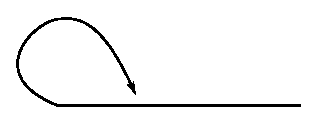
\includegraphics{1.eps}
\end{figure}\pageoriginale
The line approaches itself without touching.
\end{itemize}
\end{remarks*}

\eject

\subsection*{Submersions}

Let $f:M\to N$ be a smooth map. We say that $f$ is a submersion at a point $a\in M$ if $T_{a}(f):T_{a}(M)\to T_{f(a)}(N)$ is surjective. The map $f$ is said to be a submersion if it is a submersion at every point of $M$.

\subsection*{Theorem (Implicit function theorem) \thnum{7.2}.\label{sec7-thm7.2}}

{\em Let $f:M\to N$ be a submersion at $a\in M$. (Let $n=\dim M$ and $q=\dim N$). There exists charts $(U,\phi)$, $(V,\psi)$ for respectively $M$ and $N$, with $a\in U$, $f(a)\in V$, $f(U)\subset V$, $\varphi(a)=0\in \mathbb{R}^{n}$, $\psi\circ f(a)=0\in \mathbb{R}^{q}$ with commutativity in the diagram}
\[
\xymatrix@=1.2cm{
U\ar[d]^{\phi}\ar[r]^{f} & V\ar[d]^{\psi}\\
\varphi(U)\ar[r]_{F} & \psi(V)
}
\]
{\em where $F$ is (the restriction of) the map }
$$
\mathbb{R}^{n}\to \mathbb{R}^{q}(x_{1},\ldots,x_{n})\mapsto (x_{1},\ldots,x_{q}).
$$

It follows that a submersion is an open map.

\section{Frobenius Theorem on Integrable Sub-Bundles, Foliations}\label{sec8}

\subsection*{Sub and quotient bundles of a vector bundle}\pageoriginale

Let $E$ be a vector bundle of rank $m$ over $M$. Suppose that $F$ is a subset of $E$ which satisfies the following conditions:
\begin{itemize}
\item[(i)] for $a\in M$ the set $F_{a}=E_{a}\cap F$ is a vector subspace of dimension $p$ (fixed) of the fibre $E_{a}=\pi^{-1}(a)$ of $E$ over $a$.

\item[(ii)] every point $a\in M$ has a neighbourhood $U$ and a frame $(\sigma_{1},\ldots,\sigma_{m})$ of $E$ over $U$ such that for every $b\in U$, $\{\sigma_{1}(b),\ldots,\sigma_{p}(b)\}$ form a base for $F_{b}$.
\end{itemize}

Then $\pi/F:F\to B$ has a natural structure of a vector bundle of rank $p$ over $M$, for which $\{\sigma_{1},\ldots,\sigma_{p}\}$ are local frames. We call $F$ a sub-bundle of $E$.

Let $F$ be a subbundle of $E$. Let $E/F=\coprod\limits_{b\in M}E_{b}/F_{b}$. Let $\eta:E\to E/F$ and $\pi_{E/F}:E/F\to M$ the natural maps. Then $\pi_{E/F}:E/F\to M$ has a structure of a vector bundle for which $(\eta\circ \sigma_{p+1},\ldots,\eta\circ\sigma_{m})$ is a frame over $U$. The bundle $E/F$ is the quotient of $E$ by $F$.

\subsection*{Integrable sub-bundles of the tangent bundle : Integral Submanifolds}

Let $F$ be a subbundle of rank $p$ of the tangent bundle $T(M)$ of $M$. A submanifold $N$ of $M$ is said to be an {\em integral manifold} for $F$ if the canonical map $T_{b}i:T_{b}(N)\to T_{b}(M)$ maps the tangent space $T_{b}(N)$ of $N$ at $b$ isomorphically onto the fibre $F_{b}$ of $F$ at $b$, for each\pageoriginale $b\in N$ (Here $i:N\to M$ is the inclusion map)

\begin{defi*}
Let $F$ be a subbundle of $T(M)$. We say that $F$ is integrable (or completely integrable) if the following condition is satisfied : if $U$ is an open set of $M$ and $X$, $Y$ sections of $F$ over $U$, then $[X,Y]$ is a section of $F$.
\end{defi*}

($X$ and $Y$ are considered as sections of $T(M)$ i.e., as vector fields and $[X,Y]$ is the bracket of vector fields which is a section of $T(M)$ and we require that $[X,Y]_{b}\in F_{b}$ for $b\in U$).

\begin{remark*}
Let $F$ be a subbundle of $T(M)$. We then have a section $\Omega$ of $({\displaystyle{\mathop{\wedge}\limits^{2}}}F^{*}\otimes (T(M)/F))$ i.e., we have for $b\in M$, an alternating bilinear map $F_{b}\times F_{b}\to (E/F)_{b}$. This is defined as follows: Let $v_{1}$, $v_{2}\in F_{b}$ and let $X$, $Y$ be vector fields (in a neighbourhood of $b$) with $x(a)=v_{1}$, $X(b)=v_{2}$. Define $\Omega(v_{1},v_{2})=\eta_{b}[X,Y]_{b}$, where $\eta_{b}:T_{b}\to T_{b}(M)/F_{b}$ is the natural map. One checks that $\Omega$ depends only on $v_{1}$, $v_{2}$ and not on the extensions $X$ and $Y$. This section $\Omega$ may be called the {\em curvature} of the subbundle $F$. Thus $F$ is integrable if and only if its curvature is identically zero.
\end{remark*}

\subsection*{Frobenius Theorem}

\begin{theorem}\label{sec8-thm8.1}
The following conditions on a subbundle $F$ of $T(M)$ are equivalent.
\begin{itemize}
\item[\rm(1)] Through every point $a\in M$, there is an integral submanifold for $F$.

\item[\rm(2)] $F$ is integrable.

\item[\rm(3)] Each point $a\in M$ has a neighbourhood $U$, a diffeomorphism $\varphi:U\to V\times W$,\pageoriginale where $V$ and $W$ are open subsets of $\mathbb{R}^{p}$ and $\mathbb{R}^{n-p}$ respectively, such that for each $w\in W$, the set $\varphi^{-1}\circ p^{-1}_{W}(w)$ ($p_{W}:V\times W\to W$ the projection) is an integral submanifold of $F$.
\[
\xymatrix@=1.2cm{
U\ar[r]^-{\phi} & V\times W\ar[d]^-{p_{W}}\\
             & W
}
\]
(In other words, around each point $a$ there exists a system of coordinates $(x_{1},\ldots,x_{n})$ for $M$ such that the submanifolds $x_{p+1}=c_{p+1},\ldots,x_{n}=c_{n}$, where $c_{p+1},\ldots,c_{n}$ are constants, are integral submanifolds of $F$.)
\end{itemize}
\end{theorem}

\begin{proof}
(3) $\Rightarrow$ (1) is trivial.
\end{proof}

To prove (1) $\Rightarrow$ (2) we use

\begin{lemma}\label{sec8-lem8.2}
Let $f:N\to M$ be a smooth map. If $X_{1}$ (resp. $X$), a vector field on $N$ (resp. $M$) we say that $X_{1}$ and $X$ are $f$-related if for each $b\in N$ we have $T_{b}(f)(X_{1}(b))=X(f(b))$. Suppose that $X_{1}$ and $Y_{1}$ vector fields on $N$ and $X$, $Y$ vector fields on $M$ such that $X_{1}$ is $f$-related to $X$ and $Y_{1}$ is $f$-related to $Y$. Then $[X_{1},Y_{1}]$ is $f$-related to $[X,Y]$.
\end{lemma}

To deduce (1) $\Rightarrow$ (2) from the lemma we take $f$ to be the inclusion $i:N\to M$, $X_{1}=X|_{N}$, $Y_{1}=Y|_{N}$.

The essential part of the proof is to show that (2) $\Rightarrow$ (3). This is done in two steps. First one proves

\begin{lemma}\label{sec8-lem8.3}
Suppose\pageoriginale that $F$ is integrable. Each point $a\in M$ has a neighbourhood of $U$ and a frame $\{X_{1},\ldots,X_{p}\}$ for $F$ over $U$ such that $[X_{i},X_{j}]=0$ for $1\leq i\leq p$, $1\leq j\leq p$.
\end{lemma}

The proof of this lemma is essentially algebraic. One then proves

\begin{proposition}\label{sec8-prop8.4}
Let $X_{1},\ldots,X_{p}$ be a vector fields in a neighbourhood $U$ of a such that $\{X_{1}(b),\ldots,X_{p}(b)\}$ are linearly independent in $T_{b}(M)$ for each $b\in U$ and such that $[X_{i},X_{j}]=0$ in $U$, for $1\leq i\leq p$, $1\leq j\leq p$. Then there exists a coordinate system $(x_{1},\ldots,x_{n})$ in a neighbourhood $V$ of a such that $X_{i}=\sigma/\partial x_{i}$, $1\leq i\leq p$ in $V$.
\end{proposition}

\subsection*{Sketch of proof of the proposition}

Choose a coordinate system $(y_{1},\ldots,y_{n})$ around $a$ with $y_{i}(a)=0$ and such that $X_{1}(a),\ldots,X_{p}(a)$, $(\partial/\partial y_{p+1})_{a},\ldots,(\partial/\partial y_{n})_{a}\text{~span~} T_{a}(M)$. Let $\varphi^{i}_{t}$ be the local flow associated with $X_{i}$, $1\leq i\leq p$. For $\delta>0$, let $\Omega=\{(t_{1},\ldots,t_{p},y_{p+1},\ldots,y_{n})\big| |t_{i}|<\delta,|y_{j}|<\delta\}$. For $\delta$ sufficiently small, the map $h:\Omega\to M$
$$
h(t_{1},\ldots,t_{p},y_{p+1},\ldots,y_{n})=\varphi^{1}_{t_{1}}\circ,\ldots,\circ\varphi^{p}_{t_{p}}(0,\ldots,0,y_{p+1},\ldots,y_{n})
$$
is well-defined. It is easy to check that
$$
T_{0}(h)\left((\partial/\partial t_{i})_{0}\right)=X_{i}(a)\text{~ and~ } T_{0}(h)\left((\partial/\partial y_{j})_{0}\right)=(\partial/\partial y_{j})_{a},
$$
so that $h$ is a diffeomorphism in a neighbourhood $V$ of $0$. Next one shows that, for $x\in V$,
$$
T_{x}(h)\left((\partial/\partial t_{i})_{x}\right)=X_{i}h(x),\quad 1\leq i\leq p.
$$
To prove this one uses the fact that $\varphi^{i}_{t}$ and $\varphi^{j}_{t}$ commute for $1\leq i\leq p$, $1\leq j\leq p$ as\pageoriginale $[X_{i},X_{j}]=0$ (see p.\pageref{page26} Corollary \ref{sec6-coro6.5.1}).

The implication (2) $\Rightarrow$ (3) is clear from the Proposition.

\subsection*{Foliatoin}
\label{page38}

Let $F$ be an integrable subbundle (of rank $p$) of $T(M)$. We define a new topology on $M$ by declaring that a subset of $M$ is open if it is a union of integral submanifolds for $F$. With this topology $M$ becomes, in a natural way, a $p$-dimensional manifold, which we denote by $M_{F}$. A connected component of $M_{F}$ is called a maximal integral manifold (or a leaf) of $F$. The leaves define a partition of $M$, called the foliation of $M$ defined by $F$. If $N$ is a leaf, note that the inclusion map $i:N\to M$ is an injective immersion; in general $N$ need not be a submanifold of $M$.

\section{Lie Groups (Continued)}\label{sec9}

\subsection*{The Lie algebra of a Lie group}

Let $G$ be a Lie group. A vector field $X$ on $G$ is said to be left invariant if for each $x\in G$ and $g\in G$ we have $X(gx)=T_{x}(L_{g})(X(x))$ where $L_{g}:G\to G$ is the left translation by $g$ i.e., $L_{g}(y)=gy$. A left invariant vector field is uniquely determined by its value at the identity element $e$ and given $v\in T_{e}(g)$ there exists a unique left invariant vector field $X$ with $X(e)=v$. Moreover, if $X$ and $Y$ are left invariant vector fields, so are $\lambda X+\lambda Y$, $(\lambda,\mu\in \mathbb{R})$ and $[X,Y]$. Thus the set of left invariant vector fields on $G$ form a $n$-dimensional ($n=\dim G$) Lie algebra over $\mathbb{R}$, called the Lie algebra of $G$ and denoted by $\mathfrak{g}$.

Let\pageoriginale $G_{1}$ and $G_{2}$ be Lie groups and $\varphi:G_{1}\to G_{2}$ a smooth homomorphism. Let $\mathfrak{g}_{1}$ (resp. $\mathfrak{g}_{2}$) be the Lie algebra of $G_{1}$ (resp. $G_{2}$). Then $\varphi$ induces a Lie algebra homomorphism $\varphi_{*}:\mathfrak{g}_{1}\to \mathfrak{g}_{2}$, as follows. Let $X\in \mathfrak{g}_{1}$ and $e_{i}(i=1,2)$ be the identity element of $G_{i}$. Let $X'\in \mathfrak{g}_{2}$ with $X'(e_{2})=T_{e_{1}}(\varphi)(X(e_{1}))$ and define $\phi_{*}(X)=X'$. Since for $g\in G$ we have $\varphi\circ L_{g}=L_{\varphi(g)}\circ \varphi$ it is easy to check that $X$ and $X'$ are $\varphi$=related. It follows from Lemma \ref{sec8-lem8.2} that $\varphi_{*}$ is a Lie algebra homomorphism.

In particular $\varphi:G_{1}\to G_{2}$ is a homomorphism which is an injective immersion, $\mathfrak{g}_{1}$ can be identified with the Lie subalgebra $\varphi_{*}(\mathfrak{g}_{1})$ of $\mathfrak{g}_{2}$.

\subsection*{Lie subalgebras and Lie subgroups}

Let $G$ be a Lie group and $H\subset G$. Suppose that $H$ has a structure of Lie group such that the inclusion map $i:H\to G$ is a homomorphism which is an injective immersion. We say that $H$ is a Lie subgroup of $G$. (A Lie subgroup $H$ need not be a submanifold of $G$; in fact if it is so, it should be closed in $G$). The Lie algebra $\mathfrak{H}$ of $H$ is identified by $i_{*}$ with a subalgebra of $\mathfrak{g}$.

\begin{proposition}\label{sec9-prop9.1}
Let $G$ be a Lie group and $\mathfrak{H}$ a Lie subalgebra of $\mathfrak{g}$. Then there exists a Lie subgroup $H$ of $G$ whose Lie algebra is $\mathfrak{H}$.
\end{proposition}

\noindent
{\bf Idea of Proof.}~ The subalgebra $\mathfrak{H}$ defines an integrable subbundle $F$ of $T(G)$ as follows. The fibre $F_{x}$ of $F$ at $x\in G$, is the subspace of $T_{x}(G)$, $\{X(x)|x\in \mathfrak{H}\}$. Since for $X$, $Y\in \mathfrak{H}$, we have $[X,Y]\in \mathfrak{H}$, $F$\pageoriginale is an integrable subbundle of $T(G)$. Let $H$ be the leaf through $e$ of the foliation on $G$ defined by $F$. One checks that $H$ is a Lie subgroup of $G$ whose Lie algebra is $\mathfrak{H}$, using that if $C$ is a leaf then $gC$ is a leaf, for $g\in G$.

\subsection*{Homomorphisms of Lie groups and Lie algebras}

Let $G_{1}$ and $G_{2}$ be two lie groups with lie algebras $\mathfrak{g}_{1}$, $\mathfrak{g}_{2}$. Then the Lie algebra of the Lie group $G_{1}\times G_{2}$ is naturally identified with the direct product $\mathfrak{g}_{1}\times \mathfrak{g}_{2}$. Let $\varphi : G_{1}\to G_{2}$ be a homomorphism of Lie groups and $\varphi_{*}:\mathfrak{g}_{1}\to \mathfrak{g}_{2}$ the induced homomorphism. The graph $\Gamma=\{(x,\varphi(x));x\in G_{1}\}$, of $\varphi$ is a (closed) Lie subgroup of $G_{1}\times G_{2}$ whose Lie algebra is the graph $\Gamma'=\{(v,\phi_{*}v);v\in \mathfrak{g}_{1}\}$ of $\varphi_{*}$. From this we deduce that if $\varphi_{1}$ and $\varphi_{2}$ are two homomorphisms of $G_{1}$ into $G_{2}$ and $\varphi_{1^{*}}=\varphi_{2^{*}}$ on $\mathfrak{g}_{1}$, then $\varphi_{1}=\varphi_{2}$ if $G_{1}$ is {\em connected}.

We now consider the question whether every homomorphism between $\mathfrak{g}_{1}$ and $\mathfrak{g}_{2}$ is induced by homomorphism between $G_{1}$ and $G_{2}$.

\begin{proposition}\label{sec9-prop9.2}
Suppose that $G_{1}$ is {\em simply connected}. If $\psi:\mathfrak{g}_{1}\to \mathfrak{g}_{2}$ is a Lie algebra homomorphism, then there exists a (unique) homomorphism $\varphi:G_{1}\to G_{2}$ such that $\varphi_{*}=\psi$.
\end{proposition}

We indicate a proof of this result.

\begin{defi*}
Let $G_{1}$ and $G_{2}$ be Lie groups and $U$ a neighbourhood of $e$ in $G_{1}$. A smooth map $f:U\to G_{1}$ is called a local homomorphism if for $x$, $y\in U$ with $xy\in U$, we have $f(xy)=f(x)f(y)$.
\end{defi*}

Using the monodromy theorem one proves:

\begin{lemma}\label{sec9-lem9.3}
Let\pageoriginale $G_{1}$ be a {\em simply connected} lie group and $f:U\to G_{2}$ be a local homomorphism where $U$ is a connected neighbourhood of $e$ in $G_{1}$. Then there exists a (unique) homomorphism (smooth) $\varphi:G_{1}\to G_{2}$ such that $\varphi|_{U}=f$.
\end{lemma}
 
To prove Proposition \ref{sec9-prop9.2}, note first that the Lie algebra of $G_{1}\times G_{2}$ is naturally isomorphic to $\mathfrak{g}_{1}\times \mathfrak{g}_{2}$, the direct product of the Lie algebras $\mathfrak{g}_{1}$ and $\mathfrak{g}_{2}$. Let $\Gamma'=\{(v,\psi(v)); v\in \mathfrak{g}_{1}\}\subset (\mathfrak{g}_{1}\times \mathfrak{g}_{2})$ be the graph of $\psi$. Then $\Gamma'$ is a subalgebra of $\mathfrak{g}_{1}\times \mathfrak{g}_{2}$. Let $\Gamma$ be a Lie subgroup of $G_{1}\times G_{2}$ corresponding to $\Gamma'$. The tangent map at identity of the restriction of the projection $\pr_{G_{1}}:G_{1}\times G_{2}\to G_{1}$ to $\Gamma$ is $(v,\psi(v))\mapsto v$, so that this map is a local diffeomorphism of a neighbourhood of identity in $\Gamma$ onto a (connected) neighbourhood $U$ of $e$ in $G_{1}$. Then the composite $f$ of the maps $(\pr_{G_{1}})^{-1}:U\to \Gamma$ and $\pr_{G_{2}}:\Gamma\to G_{2}$ is a local homomorphism. Since $G_{1}$ is simply connected, by Lemma \ref{sec9-lem9.3}, $f$ extends to a homomorphism $\varphi:G_{1}\to G_{2}$ which is the required homomorphism.

\subsection*{The exponential map}

The Lie algebra of the Lie group $\GL(n,\mathbb{R})$ can be identified with the Lie algebra $\mathfrak{g}(n,\mathbb{R})$ of $n\times n$ real matrices. If $A$ and $B$ are $n\times n$ matrices $[A,B]$ is defined to be $AB-BA$). If $A\in \mathfrak{g}(n,\mathbb{R})$, the series $I+A+A^{2}+\cdots+\dfrac{A^{n}}{n!}+\cdots$ defines an element in $\GL(n,\mathbb{R})$ denoted by $\exp A$, called the exponential of $A$. Thus $A\mapsto \exp A$ is a map of the Lie algebra of $\GL(n,\mathbb{R})$ into $\GL(n,\mathbb{R})$. We shall generalise this to any Lie group $G$.

Considering\pageoriginale $\mathbb{R}$ as a Lie group, the vector field $\dfrac{d}{dt}$ on $\mathbb{R}$ is a left invariant vector field. Let $G$ be Lie group and $X$ an element of $\mathfrak{g}$. There exists a unique Lie algebra homomorphism of the Lie algebra of $\mathbb{R}$ into $\mathfrak{g}$, sending $\dfrac{d}{dt}$ into $X$. Since $\mathbb{R}$ is simply connected, there exists a unique homomorphism $\phi_{X}:\mathbb{R}\to G$ whose tangent map is the above homomorphism. We define
\begin{equation*}
\exp X=\phi_{X}(1).\quad (1\in \mathbb{R})
\end{equation*}
We have
\begin{itemize}
\item[(1)] $\exp((t_{1}+t_{2})X)=\exp(t_{1}X)\exp(t_{2}X)$, $t_{1}$, $t_{2}\in \mathbb{R}$.

\item[(2)] $\exp(-tX)=\exp(tX)^{-1}$, $t\in \mathbb{R}$.

\item[(3)] $\exp :\mathfrak{g}\to G$ is a smooth map.

\item[(4)] $\exp$ is a local diffeomorphism at $0\in \mathfrak{g}$.
\end{itemize}

\subsection*{The adjoint representation of a Lie group}

If $V$ is a finite dimensional vector space over $\mathbb{R}$, the group $\Aut(V)$ of linear automorphisms is a Lie group (If $\dim V=m$, we can identify $\Aut V$ with $\GL(m,\mathbb{R})$ if we choose a base for $V$). A smooth homomorphism $\rho:G\to \Aut(V)$ is called a representation of the Lie group $G$ on $V$.

We shall now define a natural representation of a Lie group on its Lie algebra, called the adjoint representation of $G$. Let $g\in G$ and $\Int g : G\to G$ be the map $s\mapsto gsg^{-1}$, $s\in G$. Define $\Ad g:T_{e}(G)\to T_{e}(G)$ to be $T_{e}(\Int g)$. Identifying $T_{e}(G)$ with $\mathscr{T}$, we\pageoriginale get a representation $g\mapsto \Ad g$ on $\mathfrak{g}$. If $R_{g}:G\to G$ is the map $s\to sg$, $s\in G$, and $X\in \mathfrak{g}$, it is not hard to prove that $(R_{g})_{*}(X)=\Ad (g^{-1})(X)$.

\section{Principal Bundles and Associated Bundles}\label{sec10}

\subsection*{Principal bundles}

\label{page43}

Let $U$ be a manifold and $G$ a Lie group. We make $G$ act on $U\times G$ on the right as follows: $((x,s),g)\mapsto (x,sg)$, for $x\in U$, $s$, $g\in G$. Note that the action of $G$ is free i.e., if $y\in U\times G$ and $yg=g$, $g\in G$, then $g=e$. Moreover given $y_{1}$, $y_{2}$ with $\pr_{U}(y_{1})=\pr_{U}(y_{2})$ then there exists a unique element $g\in G$ with $y_{2}=y_{1}g$ i.e., $G$ acts simply transitively on the fibres of the map $U\times G\to U$.

We now consider the situation where a Lie group $G$ acts on a manifold $p$, where the situation is `locally' as above.

\begin{defi*}
Let $\pi:P\to M$ be a map of smooth manifolds. Suppose that a Lie group $G$ acts on the right on $P$ and that every point $x\in M$ has a neighbourhood $U$ and a diffeomorphism $\tau : U\times G\to \pi^{-1}(U)$ such that
\begin{itemize}
\item[(i)] the diagram
\[
\xymatrix{
U\times G\ar[dr]_{p_{U}}\ar[rr]^-{\tau} & & \pi^{-1}(U)\ar[dl]^{\pi}\\
 & U & 
}
\]
commutes, and

\item[(ii)] $\tau(x,sg)=\tau(x,s)g$, for $x\in P$, $s$, $g\in G$. Then we say that $P$ is\pageoriginale a principal handle over $M$ with structure group $G$, or simply that $P$ is a principal $G$-bundle over $M$.
\end{itemize}
\end{defi*}

\begin{remarks*}
\begin{itemize}
\item[(1)] $G$ acts freely on $P$.

\item[(2)] $G$ acts simply transitively on each fibre of $\pi:P\to M$.
\end{itemize}
\end{remarks*}

\subsection*{The bundle of frames associated to a vector bundle}

As an example of a principal bundle, we shall associate to a vector bundle $E$ of rank $m$ over $M$, a principal bundle over $M$ with $\GL(m,\mathbb{R})$ as structure group, called the bundle of frames of $E$. Let $P$ be the set of linear isomorphisms of $\mathbb{R}^{m}$ into the fibres of $E$ (If $\varphi:\mathbb{R}^{m}\to E_{x}$ is an isomorphism and $(e_{1},\ldots,e_{m})$ is the canonical basis in $\mathbb{R}^{m}$, then $(\varphi(e_{1}),\ldots,(e_{m}))$ is a basis in $E_{x}$; conversely given a basis $(f_{1},\ldots,f_{m})$ of $E_{x}$ there exists a unique isomorphism of $\mathbb{R}^{m}$ into $E_{x}$ sending $e_{i}$ into $f_{i}$. Thus $P$ can be identified with the set of basis (`frames') in the different fibres of $E$. This explains the terminology). We make $\GL(m,\mathbb{R})$ act on $P$ as follows: if $x\in M$, $\varphi:\mathbb{R}^{m}\to E_{x}$ an isomorphism and $g\in \GL(m,\mathbb{R})$, then $((x,\varphi),g)\mapsto (x,\varphi\circ g)$, $g$ being considered as an isomorphism $\mathbb{R}^{m}\to \mathbb{R}^{m}$. $P$ has a natural structure of a manifold (in fact it is an open subset of $E\otimes\cdot\otimes E$, $m$ times) and becomes a principal $\GL(m,\mathbb{R})$ bundle under this action.

Note that if there is a smooth section of $P$ (i.e., a smooth map $\sigma:M\to P$, with $\pi\circ \sigma=\Iid_{M}$) the vector bundle $E$ is trivial.

\subsection*{Morphisms of bundles. Gauge transformations}

Let $P$ and $P'$ be principal $G$-bundles over $M$ and $M'$ respectively. A morphism or a bundle homomorphism from $P$ to $P'$ is a smooth\pageoriginale map $h:P\to P'$ such that $h(pg)=h(p)\cdot g$, for $p\in p$ and $g\in G$.

It is easily seen that $h$ induces a smooth map $\underline{h}:M\to M'$ such that the diagram
\[
\xymatrix@=1.5cm{
P\ar[d]^{\pi}\ar[r]^{h} & P'\ar[d]^{\pi'}\\
M\ar[r]_{\underline{h}} & M'
}
\]
commutes.

If $M=M'$ and if there is a morphism $h:P\to P'$ such that the induced map $\underline{h}:M\to N$ is the identity we say that $P$ and $P'$ are isomorphic. (In this case it is easy to see that $h:P\to P'$ is bijective and $h^{-1}:P'\to P$ is a morphism).

If $P$ is a principal $G$-bundle over $M$, a morphism of $P$ into $P$, which induces identity on the base is called a gauge transformation (such a morphism is an automorphism of $P$). The gauge transformations of $P$ form a group, called the group of gauge transformations of the principal, bundle $G$.

A bundle isomorphic to the trivial bundle $M\times G$ is called trivial.

\begin{proposition}\label{sec10-prop10.1}
Let $P$ be a principal $G$ bundle over $M$. Then the following conditions are equivalent.
\begin{itemize}
\item[\rm(1)] $P$ is trivial.

\item[\rm(2)] There exists a smooth section $\sigma:M\to P$.
\end{itemize}
\end{proposition}

\begin{proof}
(1)\pageoriginale $\Rightarrow$ (2) is clear, since the trivial bundle admits for instance the section $x\mapsto (x,e)$. To prove (2) $\Rightarrow$ (1) let $h'(P)$ be the unique element in $G$ such that $\sigma(\pi(p))h'(p)=p$, for $p\in P$. Then $h:P\to M\times G$ defined by $h(p)=(\pi(p),h'(p))$ is an isomorphism of $G$-bundles.
\end{proof}

\subsection*{Associated bundles}

Let $P$ be a principal $G$-bundle over $M$ and $F$ a manifold with a left action of $G$. Consider the action of $G$ on $P\times F$ given by:
$$
((p,f),g)\mapsto (pg,g^{-1}f).
$$
One can show that $P\times F$ is a principal $G$-bundle over the quotient space $(P\times F)/G$. We denote $(P\times F)/G$ by $\fprod{P}{F}{G}$. The map $(p,f)\mapsto \pi(p)$ induces a map $\fprod{P}{F}{G}\to M$, which is called the bundle associated to $P$ by the action of $G$ on $F$. If $p\in P$, $p$ induces a diffeomorphism of $F$ with the fibre over $\pi(p)$ of the map $\fprod{P}{F}{G}\to M$.

Any structure on $F$ invariant under the action can be put on the fibres of the associated bundle.

As an example let $F$ be a finite dimensional vector space and $\rho:G\to \Aut(F)$ be a (smooth) homomorphism so that $G$ acts on $F$ by linear transformations. Then $\fprod{P}{F}{G}$ is a vector bundle over $M$, called the vector bundle associated to the representation $\rho$. 

\subsection*{Extension and restriction of the structure group}
\pageoriginale

Let $P$ be a principal $G_{1}$ bundle and $\rho:G_{1}\to G_{2}$ a homomorphism of Lie groups. We can then define a principal $G_{2}$-bundle over $M$, as follows. $G_{1}$ operates on $G_{2}$ by $(g_{1},g_{2})\mapsto \rho(g_{1})\cdot g_{2}$, $g_{i}\in G_{i}$. The action of $G_{2}$ on $P\times G_{2}$ given by $(p,s)s'=(p,ss')$, $p\in P$, $s$, $s'\in G_{2}$ goes over into an action of $G_{2}$ on the associated bundle $\fprod{P}{G_{2}}{G_{1}}$ and makes of it a principal $G_{2}$ bundle. This $G_{2}$ is bundle is said to be obtained by extension of the structure group by $\rho$.

Suppose that $H$ is a Lie subgroup of $G$ and $P$ a $G$-bundle over $M$. If there exists an $H$-principal bundle $Q$ over $M$ such that the $G$-bundle, obtained from $Q$ by extension of the structure group by the inclusion map $H\to G$, is isomorphic to $P$ (as a $G$-bundle), we say that the structure group of $P$ can be reduced to $H$.

\subsection*{The pull-back (or inverse image) of a bundle}

Let $P$ be a principal $G$-bundle over $M$ and $f:N\to M$ be a smooth map of manifolds. Let $\fprod{P}{M}{N}$ be the subset of $P\times N$ consisting of points $(p,y)$ with $\pi(p)=f(y)(p\in P,y\in N)$. $G$ acts on $\fprod{P}{M}{N}$ by $(p,y)g=(pg,y)$. With this action $\fprod{P}{M}{N}$ becomes a principal $G$-bundle on $N$, called the pull-back of $P$ by $f$ (and sometimes denoted by $f^{*}(P)$). We have a commutative diagram
\[
\xymatrix@=1.5cm{
f^{*}(P)\ar[r]\ar[d] & P\ar[d]^{\pi}\\
N\ar[r]_-{f} & M
}
\]
(The\pageoriginale maps $f^{*}(P)\to P$ and $f^{*}(P)\to N$ are given by the restrictions of the projections of $P\times N$ onto $P$ and $N$ respectively.)

\section{Equivariant Forms on a Principal Bundle}\label{sec11}

{\bf The tangent bundle along the fibres of a principal bundle. Vertical vectors.}

Let $\pi:P\to M$ be a principal bundle with structure group $G$. Let $P\in p$. We denoted by $V_{p}$ the kernel of the map $T_{p}(\pi):T_{p}(P)\to T_{\pi(p)}(M)$. An element of $V_{p}$ is called a vertical vector at $p$. The tangent space at $p$ of the fibre of $\pi$ through $p$ can be identified with $V_{p}$. The vertical vectors $\coprod\limits_{p\in P}V_{p}$ form a subbundle of $T(P)$, called the tangent bundle along the fibres of $P$, denoted by $T_{\pi}$ or $V$.

\begin{proposition}\label{sec11-prop11.1}
The tangent bundle along the fibres of $P$ is trivial. More precisely there is a canonical isomorphism $\psi$ of the trivial vector bundle $P\times \mathfrak{g}$ with $T_{\pi}$ with the following property: for each $g\in G$ the diagram
\[
\xymatrix@=1.5cm{
P\times \mathfrak{g}\ar[d]^{R_{g}\times \Ad (g^{-1})}\ar[r]^-{\psi} & T_{\pi}\ar[d]^{(R_{g})_{*}}\\
P\times \mathfrak{g}\ar[r]_{\psi} & T_{\pi}
}
\]
is commutative. Here $(R_{g})_{*}$ is the `differential map' induced by the diffeomorphism $R_{g}$, $q\mapsto gg$, $q\in P$ (If $\eta:T_{\pi}\to P$ is the projection and $v\in T_{\pi}$, $(R_{g})_{*}(v)=T_{\eta(v)}(R_{g})(v)$). If $p\in P$, $\xi\in \mathfrak{g}$, $\Iid\times \Ad (g^{-1})(p,\xi)=(p,\Ad(g^{-1})\xi)$)
\end{proposition}

\noindent
{\bf Indication of proof.}\pageoriginale If $p\in P$, consider the orbit map $\sigma_{p}:G\to P$. Note that $\sigma_{p}(e)=p$. The tangent map of $\sigma_{p}$ at $e$ maps $\mathfrak{g}=T_{e}(G)$ isomorphically onto $V_{p}$. These isomorphisms, as $p$ varies, give $\psi$. The commutativity of the diagram can be proved using
\begin{itemize}
\item[(i)] if $X\in \mathfrak{g}$ and $R_{g}:G\to G$ is the right translation we have $(R_{g})_{*}(X)=\Ad(g^{-1})(X)$ (see p.\ref{page43})

\item[(ii)] commutativity of the diagram
\[
\xymatrix@=1.5cm{
G\ar[d]^{R_{g}} \ar[r]^{p} & P\ar[d]^{R_{g}}\\
G\ar[r]^{p} & P
}
\]

\end{itemize}

\begin{remark}\label{sec11-rem11.2}
If $X\in \mathfrak{g}$, $X$ defines in natural way a section of the trivial bundle $P\times \mathfrak{g}$, $p\mapsto (p,x)$. Using the isomorphism $\psi$, we get a section of $T_{\pi}$, and hence a vertical vector field, denoted by $\sigma(X)$ and called the fundamental vector field on $P$ defined by $X$. If $X$, $Y\in \mathfrak{g}$, we have $\sigma[X,Y]=[\sigma(X),\sigma(Y)]$. From the commutativity of the diagram in the Proposition, we have: $(R_{g})_{*}\sigma(X)$ is the fundamental vector field corresponding to $\Ad(g^{-1})(X)\in \mathfrak{g}$.
\end{remark}

\subsection*{Alternating forms with values in a vector space}

Let $E$ and $F$ be finite dimensional vector spaces over $\mathbb{R}$. It is clear how to define an alternating $p$-form on $E$ with values in $F$. For instance a $2$-form is a bilinear map $f:E\times E\to F$ with $f(x,x)=0$ for $x\in E$. Let $F_{1}$, $F_{2}$, $F_{3}$ be (finite dimensional) vector\pageoriginale spaces and $\varphi:F_{1}\times F_{2}\to F_{3}$ a bilinear map. If $\alpha$ (resp. $\beta$) is a $p$ (resp. $q$) form on $E$ with values in $F_{1}$ (resp. $F_{2}$) we can define $\varphi(p+q)$ form on $E$ with values $F_{3}$, as on page \pageref{page13}, using $\varphi$ instead of multiplication in $\mathbb{R}$, (We denote this form by $\alpha\wedge_{\varphi}\beta$). For instance if $p=q=1$, $(\alpha\wedge_{\varphi}\beta)(X,Y)=\varphi(\alpha(X),\beta(Y))-\varphi(\alpha(Y),\beta(X))$ for $X$, $Y\in E$.

Consider the special case $F_{1}=F_{2}=F_{3}=\mathfrak{g}$, where $\mathfrak{g}$ is a Lie algebra and $\varphi:\mathfrak{g}\times \mathfrak{g}\to \mathfrak{g}$ is the map $\varphi(X,Y)=[X,Y]$, $X$, $Y\in \mathfrak{g}$. In this case we denote $\alpha\wedge_{\varphi}\beta$ by $[\alpha,\beta]$. Note that if $\alpha$ is a $1$-form with values in $\mathfrak{g}$, we have
\begin{align*}
[\alpha,\alpha](X,Y) &= [\alpha(X),\alpha(Y)]-[\alpha(Y),\alpha(X)]\\[3pt]
                     &= 2[\alpha(X),\alpha(Y)]
\end{align*}
We have 
\begin{itemize}
\item[(i)] $[\alpha,\beta]=(-1)^{pq+1}[\beta,\alpha]$\label{page50}

\item[(ii)] If $\gamma$ is a $r$-form with values in $\mathfrak{g}$,
$$
(-1)^{\pr}[\alpha,[\beta,\gamma]]+(-1)^{qp}[\beta,[\gamma,\alpha]]+(-1)^{rq}[\gamma,[\alpha,\eta]]=0.
$$
\end{itemize}

It is clear that we can define on a manifold $M$ smooth differential forms with values in a vector space (finite dimensional) $F$. If $\alpha$ is such a smooth $p$-form on $M$, we can define the exterior differential $d_{\alpha}$, which is a $(p+1)$ form with values in $F$. If we wish, we can define $d$ by the analogue of the formula in Prop.\ref{sec6-prop6.6}(p.\pageref{page30}) for $d$. In particular if $\alpha$ is a $1$-form with values in $F$, $d\alpha(X,Y)=X\alpha(Y)-Y\alpha(X)-\alpha[X,Y]$,\pageoriginale $X$, $Y$ being vector fields on $M$.

In the case $F=\mathfrak{g}$, a Lie algebra for differential forms $\alpha$, $\beta$, $\gamma$ with values in $\mathfrak{g}$ we have (i), (ii) above and 
$$
d[\alpha,\beta]=[d\alpha,\beta]+(-1)^{p}[\alpha,d\beta].
$$

\subsection*{The Maurer-Cartan form and equation}

We give an illustration of the above notion. Let $G$ be a Lie group with Lie algebra $\mathfrak{g}$. Then there is a canonical $1$-form on $G$ with values in $\mathfrak{g}$, called the Maurer-Cartan form on $G$. this form $\alpha$ is defined as follows. Let $v$ be a tangent vector of $G$ at $g$. There exists a unique left invariant vector field $X$ on $G$ with $X(g)=v$. Define $\alpha(v)=X$. Note that $\alpha$ is essentially the identity map on $T_{e}(G)$.

\medskip

\noindent
{\bf Proposition (Maurer-Cartan equation) \thnum{11.3}.\label{sec11-prop11.3}}

{\em We have $d\alpha+\dfrac{1}{2}[\alpha,\alpha]=0$.}

\begin{proof}
Let $X$ and $Y$ be left invariant vector fields. Noting that 
$$
\dfrac{1}{2}[\alpha,\alpha](X,Y)=[\alpha(X),\alpha(Y)],
$$ 
it suffices to show that $d\alpha[X,Y]+[\alpha(X),\alpha(Y)]=0$. But
\begin{align*}
d\alpha(X,Y) &= X\alpha(Y)-Y\alpha(X)-\alpha[X,Y]\\[3pt]
             &= -\alpha[X,Y],\text{~ as~ }\alpha(Y)=Y, \ \alpha(X)=X\text{~ are constants}\\[3pt]
             &= -[X,Y]=-[\alpha(X),\alpha(Y)].
\end{align*}
\end{proof}

\subsection*{Equivariant forms on principal bundles}
\pageoriginale

Let $\rho:G\to\Aut (F)$ be a finite dimensional representation of $G$. Let $\alpha$ be a $p$-form on $P$ with values in $F$. We say that $\alpha$ is equivariant (with respect to $\rho$) if $R^{*}_{g}\alpha=\rho(g^{-1})\alpha$\footnote[2]{$R^{*}_{g}\alpha$ is the inverse image of $\alpha$ by the map $R_{g}$, $p\mapsto pg$.}. (Here $\rho(g^{-1})\alpha^{-}$ is the $p$-form on $P$ defined by 
$$
[\rho(g^{-1})\alpha](X_{1},\ldots,X_{p})=\rho(g^{-1})\alpha(X_{1},\ldots,X_{p})\text{~ for~ } X_{1},\ldots,X_{p}
$$
tangent vectors on $P$. For $p=0$, the condition means $\alpha(pg)=\rho(g^{-1})\alpha(p)$, $p\in P$, $g\in G$, $\alpha$ being a function from $P$ to $V$). Since $dR^{*}_{g}=R^{*}_{g}d$, we see that if $\alpha$ is an equivariant $p$-form then $d$ is an equivariant $(p+1)$ form.

An equivariant $p$-form is said to be basic (``coming from the base'') or horizontal if $\alpha(X_{1},\ldots,X_{p})=0$ if at least one of the tangent vectors $X_{i}$ is vertical. Basic equivariant $p$-forms can be identified with the sections of the bundle ${\displaystyle{\mathop{\wedge}\limits^{p}}}T^{*}(M)\otimes F_{\rho}$ on $M$, where $F_{\rho}$ is the vector bundle on $M$ associated to the representation $\rho$. Hence such forms are also called $p$-forms {\em on $M$} with coefficients in the bundle $F_{\rho}$. In particular applying this to the case of the trivial $1$-dimensional representation of $G$, we see that a $p$-form (in the usual sense) on $M$ can be identified with a $p$-form $\alpha$ on $P$ which is invariant under the action of $G$ and which satisfies $\alpha(X_{1},\ldots,X_{p})=0$ if one of the $X_{i}$ is vertical.

Note that if $\alpha$ is basic, the form $d\alpha$, while being equivariant need not be basic.

\section{Connection and Curvature}\label{sec12}

\subsection*{Connections and connection forms}
\pageoriginale

\begin{defi*}
Let $P$ be a principal $G$-bundle. Let $T(P)$ be the tangent bundle of $P$ and $T_{\pi}$ the tangent bundle along the fibres. A connection on $P$ is a subbundle $\mathscr{H}$ of $T(P)$ which is supplementary to $T_{\pi}$ and which is invariant under the action of $G$ on $T(P)$.
\end{defi*}

Thus if $\mathscr{H}_{P}$ is the fibre of $\mathscr{H}$ at $P$ we have 
\begin{center}
(a)~ $T_{p}(P)=\mathscr{H}_{p}\oplus V_{p}$\qquad (b)~ for $g\in G$, $p\in G$,
\end{center}
$T_{p}(R_{g})(\mathscr{H}_{p})=\mathscr{H}_{pg}$. An element of $\mathscr{H}$ is called an horizontal vector and $\mathscr{H}_{p}$ is called the horizontal space at $p$.

If $\eta:T(P)\to T_{\pi}$ is the projection defined by the decomposition $T(P)=\mathscr{H}\oplus T_{\pi}$ we can consider $\eta$ as a $1$-form on $P$ with values in $\mathfrak{g}$, using the isomorphism of $T_{\pi}$ with $P\times \mathfrak{g}$. We denote this $1$-form by $w$ and call it the connection form (of the connection).

Thus the form $w$ is defined as follows. Let $v\in T_{p}(P)$. Write $v=v_{1}\oplus h$ with $v_{1}\in V_{p}$, $h\in \mathscr{H}_{p}$. Under the isomorphism of $V_{p}$ with $\mathfrak{g}$, $v_{1}$ corresponds to an element $v'_{1}$ in $\mathfrak{g}$. Then we define $w(v)$ to be $v'_{1}$.

If $w_{p}:T_{p}(P)\to \mathfrak{g}$ is the value of $w$ at $p$, note that the kernel of $w_{p}$ is $\mathscr{H}_{p}$.

The\pageoriginale connection form $w$ satisfies the following two conditions.
\begin{itemize}
\item[(1)] If $x_{0}$ is a vertical vector at $p$, $w(X_{0})$ is that element $x'_{0}$ of $\mathfrak{g}$ whose associated fundamental vector field $\sigma(X'_{0})$ takes the value $X_{0}$ at $p$.

\item[(2)] $(R_{g})^{*}w=(\Ad g^{\tau l})(w)$.
\end{itemize}

These properties follow immediately from Proposition \ref{sec11-prop11.1}.

Note that the second condition means that $w$ is an equivariant $1$-form on $P$ with respect to the adjoint representation of $G$ on its Lie algebra.

Conversely given a $1$-form $w$ on $P$ with values in satisfying (1) and (2) above it defines a unique connection whose associated $1$-form is $w$. In fact define $\mathscr{H}_{p}=$ kernel of $w_{p}:T_{p}\to \mathfrak{g}$, where $w_{p}$ is the value of $w$ at $p$.

Often we do not distinguish between a connection and the associated connection form.

If $P'$ is a $G$-bundle over $M'$ and $h:P'\to P$ is a bundle homomorphism and $w$ a connection form on $P$, it is immediate that $h^{*}(w)$ is a connection form on $P'$, called the inverse image of $w$ by $h$.

\subsection*{The curvature form of a connection}

Let $P$ be a $G$-bundle with a connection. Let $\rho:G\to \Aut(F)$ be a representation of $G$. If $\alpha$ is an equivariant $p$-form (with respect to\pageoriginale $\rho$), the form $\alpha\circ H$, where $H:T(P)\to \mathscr{H}$ is the projection onto with respect to the decomposition $T(P)=\mathscr{H}\oplus T_{\pi}$, is an equivariant form which is clearly {\em basic}. (Note that if $X_{1},\ldots,X_{p}$ are tangent vectors at point of $P$, $\alpha\circ H(X_{1},\ldots,X_{p})=\alpha(HX_{1},\ldots,HX_{p})$ where $H$ is the projection on to the horizontal space). We define
$$
dw(\alpha)=d\alpha\circ H.
$$
i.e., $d_{w}(\alpha)$ is the basic form of degree $(p+1)$ associated to $d\alpha$.

\begin{defi*}
The $2$-form $d_{w}(w)$ with values in $\mathfrak{g}$ is defined to be the curvature form of the connection. It is denoted by $\Omega$.
\end{defi*}

\begin{remark}\label{sec12-rem12.1}
(1) $\Omega(X_{1},X_{2})=dw(HX_{1},HX_{2})$ (by definition) where $X_{1}$, $X_{2}$ are tangent vectors at a point of $P$.
\end{remark}

\noindent
{\bf \thnum{12.2}.\label{sec12-ref12.2}}~The curvature form is a {\em basic} 2-form with values in $\mathfrak{g}$, equivariant with respect to the adjoint representation. As such it can be identified with a $2$-form on $M$ with coefficients in the vector bundle associated to the adjoint representation. (This bundle is called the adjoint bundle of $P$).

\subsection*{Proposition (Structure equation) \thnum{12.3}.\label{sec12-prop12.3}}

{\em We have $\Omega=dw+\dfrac{1}{2}[w,w]$ where $\Omega$ is the curvature form of the connection and $w$ the connection form.}

\begin{proof}
It suffices to prove that $\Omega(X_{0},Y_{0})=dw(X_{0},Y_{0})+\dfrac{1}{2}[w,w](X_{0},Y_{0})$ in the following $3$ cases 
\begin{itemize}
\item[(1)] $X_{0}$, $Y_{0}$ are both horizontal vectors

\item[(2)] $X_{0}$, $Y_{0}$ are both vertical

\item[(3)] $X_{0}$ vertical and $Y_{0}$ horizontal.
\end{itemize}
\end{proof}

\noindent
{\bf Case \thnum{1}.\label{sec12-case1}} $X_{0}$,\pageoriginale $Y_{0}$ both horizontal. Since $w(X_{0})=w(Y_{0})=0$, we have $\dfrac{1}{2}[w,w](X_{0},Y_{0})=0$. Hence
$$
(X_{0},Y_{0})=dw(HX_{0},HY_{0})=dw(X_{0},Y_{0})=dw(X_{0},Y_{0})+\dfrac{1}{2}[w,w](X_{0},Y_{0}).
$$

\noindent
{\bf Case \thnum{2}.\label{sec12-case2}}
$X_{0}$, $Y_{0}$ both vertical vectors at $p$. The proof is similar to that of the Maorer-Cartan equation. Let $A$, $B\in \mathfrak{g}$ be such that, if $X=\sigma(A)$, $Y=\sigma(B)$ be the associated fundamental vector fields on $P$, we have $X(p)=X_{0}$, $Y(p)=Y_{0}$. Then $w(X_{0})=A$, $w(Y_{0})=B$. Since $\sigma[A,B]=[\sigma(A),\sigma(B)]$, we have $w([X,Y]_{p})=[A,B]$. Note that $\dfrac{1}{2}[w,w](X_{0},Y_{0})=[w(X_{0}),w(Y_{0})]=[A,B]$.

\smallskip
Now, since $HX_{0}=HY_{0}=0$, one has $\Omega(X_{0},Y_{0})=0$. On the other hand,
\begin{align*}
dw(X_{0},Y_{0}) &= X_{0}w(Y)-Y_{0}w(X)-w([X,Y]_{p})\\[3pt]
              &= X_{0}B-Y_{0}A-w([X,Y]_{p})\\[3pt]
              &= -[A,B]\quad(\text{as~ } B\text{~ and~ } A\text{~ are constant})\\[3pt]
              &= -\dfrac{1}{2}[w,w](X_{0},Y_{0})
\end{align*}

\noindent
{\bf Case \thnum{3}.\label{sec12-case3}}
$X_{0}$ vertical, $Y_{0}$ horizontal at $p$. Let $A$ and $X$ be as in case \ref{sec12-case2}. It is easy to see that there exists a neighbourhood $U$ of $\pi(p)$ and a horizontal vector field $Y$ on $\pi^{-1}(U)$ invariant under the action of $G$ and such that $Y(p_{0})=Y_{0}$. We then have $[X,Y]=0$ on $\pi^{-1}(U)$. In face the vector field associated to the $1$-parameter group $\varphi_{t}=R_{\exp(tA)}$ is $X$ and $(\varphi_{t})_{*}(Y)=Y$. Hence the Lie derivative $\theta_{X}(Y)$ is zero which means that $[X,Y]=0$ (see Theorem \ref{sec6-thm6.5}).

Now,\pageoriginale since $H(X_{0})=0$, we have $\Omega(X_{0},Y_{0})=0$. On the other hand
\begin{align*}
dw+\dfrac{1}{2}[w,w] &= X_{0}w(Y)-Y_{0}w(X)-w([X,Y]_{p})+[w(X_{0}),w(Y_{0})]\\[3pt]
                     &=0
\end{align*}
since $w(Y)=0$ ($Y$ being horizontal), $w(X)=A$, $[X,Y]_{p}=0$ and $w(Y_{0})=0$. This completes the proof of the structure equation. 

\setcounter{theorem}{3}
\begin{remark}\label{sec12-rem12.4}
If $X$ and $Y$ are horizontal vector fields, we have
\begin{align*}
\Omega(X,Y) &= \left(dw+\dfrac{1}{2}[w,w]\right)(X,Y)\\[3pt]
            &= Xw(Y)-Yw(X)-w[X,Y]+[w(X),w(Y)]\\[3pt]
            &= -w[X,Y]\text{~ since~ } w(X)=w(Y)=0.
\end{align*}
Thus the horizontal bundle $\mathscr{H}$ is integrable (as a subbundle of $T(P)$) if and only the curvature form is zero. A connection with curvature form is zero said to be flat. The curvature form measures the obstruction for the horizontal bundle to be integrable.
\end{remark}

\subsection*{Covariant differentiation of forms with values in associated vector bundles}

Let $\rho:G\to \Aut(F)$ be a representation. Let $\alpha$ be a $p$-form on $P$ with values $F$, which is a basic form of type $\rho$. We define a basic $(p+1)$ form, $d_{w}\alpha$, of type $\rho$ by $d_{w}\alpha=d\alpha\circ H$. Thus $d_{w}\alpha(X_{1},\ldots,X_{p+1})=d\alpha(HX_{1},\ldots,HX_{p+1})$. The form $d_{w}$ is the covariant differential of $\alpha$ with respect to the connection.

We shall now give an explicit formula for the covariant differential. For this we observe that $\rho:G\to \Aut F$ defines a linear map\pageoriginale $\rho':\mathfrak{g}\to \End F$, where $\End F$ is the vector space of endomorphisms of $F$, as follows. If $A\in \mathfrak{g}$, $v\in F$, we define
$$
\rho'(A)v=\lim\limits_{t\to 0}\dfrac{\rho(\exp tA)v-v}{t}\in V.
$$
The map $\rho'$ may be viewed as a bilinear map, still denoted by $\rho'$, $\rho':\mathfrak{g}\times F\to F$.

\begin{proposition}\label{sec12-prop12.5}
If $\alpha$ is a basic $p$-form of type $\rho$, we have
$$
dw\alpha=d\alpha+w\wedge_{\rho}, \alpha,
$$
where the exterior product is formed using the bilinear map $\rho':\mathfrak{g}\times F\to F$, noting that $w$ is a form with values in $\mathfrak{g}$ and $\alpha$ a form with values in $F$.
\end{proposition}

We shall not prove this proposition here. It may be proved by a method similar to that used in the proof of the structure equation.

\subsection*{Bianchi and Ricci identities}

\noindent
{\bf Proposition (Bianchi identity) \thnum{12.6}.\label{sec12-prop12.6}}
{\em Let $\Omega$ be the curvature form of a connection $w$. Then $d_{w}\Omega=0$ (The covariant differential of the curvature form is zero).}

\begin{proof}
We use the above formula for the covariant differential. In this case $\rho$ is the adjoint representation and the map $\rho':\mathfrak{g}\times \mathfrak{g}\to \mathfrak{g}$ is given by $(A,B)\to [A,B]$. We have
\begin{align*}
dw\Omega &= d\Omega+[w,\Omega]\\[3pt]
         &= d\left(dw+\dfrac{1}{2}[w,w]\right)+\left[w,dw+\dfrac{1}{2}[w,w]\right]\\[3pt]
         &= \dfrac{1}{2}[dw,w]-\dfrac{1}{2}[w,dw]+[w,dw]+\dfrac{1}{2}[w,[w,w]]\\[3pt]
         &= \dfrac{1}{2}[w,[w,w]]\\[3pt]
         &= 0.
\end{align*}
We\pageoriginale have used relation (i), (ii) on p.\pageref{page50} and the relation $d[\alpha,\beta]=[d\alpha,\beta]+(-1)^{p}[\alpha,d\beta]$, for a $p$ form $\alpha$.
\end{proof}

\noindent
{\bf Proposition (Ricci identity) \thnum{12.7}.\label{sec12-prop12.7}}
{\em If $\alpha$ is a basic $p$-form of type $\rho$, we have}
$$
d^{2}_{w^{\alpha}}=\Omega\wedge_{\rho}\alpha.
$$
We omit the proof.

\section{Chern-Weil Theory}\label{sec13}

Let $G$ be a Lie group with Lie algebra $\mathfrak{g}$. Let $Q$ be a homogeneous polynomial of degree $k$ on, which is invariant under the adjoint action of $G$ on $\mathfrak{g}$. (For example if $G=\GL(m,\mathbb{C})$, $\mathfrak{g}=\mathfrak{g}\ell(n,\mathbb{C})$, we take, for $A\in \mathfrak{g}\ell(n,\mathbb{C})$, $Q(A)=\text{trace~}A$, $Q(A)=\det A$ and more generally $Q(A)=k^{\text{th}}$ elementary symmetric function of the eigen-values of $A$).

Let $G$ be a principal $G$-bundle with base $M$. Let $w$ be a connection on $P$ and $\Omega$ its curvature. We shall now define a {\em closed} form of degree $2k$ on $M$, by `substituting' the curvature form in the polynomial $Q$. The form $\Omega$ being a $2$-form on $P$ with values in $\mathfrak{g}$, it defines a $2k$-form with values in $\bigotimes\limits^{k}\mathfrak{g}=\mathfrak{g}\otimes\cdots\otimes \mathfrak{g}$ ($k$ times). Composing this with $Q$, which can be considered as a linear map $\bigotimes\limits^{k}\mathfrak{g}\to \mathbb{R}$, we get a basic $2k$-form $\alpha$ on $P$, which is invariant under $G$, since $\Omega$ is basic and $Q$ is invariant under the adjoint action. Using Bianchi's identity one can show that $\alpha$ is a closed form. Now $\alpha$ can be considered as an (ordinary) form of degree $2k$ on $M$, still denoted by $\alpha$; the form $\alpha$ is closed and hence\pageoriginale defines an element of the de Rham Cohomology group $H^{2k}_{DR}(M)$.

\begin{theorem}\label{sec13-thm13.1}
The\pageoriginale class of $\alpha$ in $H^{2k}_{DR}(N)$ depends only on the polynomial $Q$ and the bundle $P$ and not on the connection $w$.
\end{theorem}

\begin{proof}
(See Reference \cite{key3}, page 226, Remark).
Since homotopic maps induce the same map on de Rham cohomology groups (Theorem \ref{sec4-thm4.2}), it is enough to show that, given two connection forms $w_{1}$ and $w_{2}$ on $P$, they are inverse images of the same connection form $\gamma$ on a principal $G$-bundle $P'$ over $M'$, by a bundle homomorphism $P\to P'$ whose projections onto $M$ (maps from $M$ to $M'$) are homotopic. (Note that the curvature form of the inverse image of a connection is the inverse image of the curvature form and that substitution of the curvature form in $Q$ is `functorial').

We take for $P'$ the principal $G$-bundle $P'=P\times \mathbb{R}$ on $M\times \mathbb{R}$ and for $\gamma$ the connection form $\gamma_{(p,t)}=tq^{*}(w_{2})+(1-t)q^{*}w_{1}$, $p\in p$, $t\in \mathbb{R}$ and $q:P\times \mathbb{R}\to P$ the projection onto $P$. It is clear that the inverse images by the inclusions $p\mapsto (p,0)$ and $p\mapsto (p,1)$ (which are $G$-morphisms) of $P$ in $P\times \mathbb{R}$ are $w_{1}$ and $w_{2}$ respectively and the projections of these inclusions onto the base (namely the maps $M\to M\times \mathbb{R}$, $x\to (x,0)$ and $x\to (x,1)$) are clearly homotopic.
\end{proof}

\begin{remark}\label{sec13-rem13.2}
The element of $H^{p}_{DR}(M)$ defined by $Q$ is called the {\em characteristic class} of $P$ corresponding to $Q$.
\end{remark}

\vskip 1cm

\appendix

\begin{center}
{\huge\bfseries Appendix}
\end{center}
\addcontentsline{toc}{section}{Appendix}

\setcounter{section}{0}
\section{Theorem (smooth partition of unity)}\label{sec13-app-sec1}

Let $M$ be a smooth (paracompact) manifold. Let $\{U_{i}\}_{i\in I}$ be an open covering of $M$. Then there exist smooth functions $\varphi_{i}:M\to \mathbb{R}$ such that
\begin{itemize}
\item[(1)] $\varphi_{i}(x)\geq 0$ ~ for ~ $x\in M$

\item[(2)] The support of the function $\varphi_{i}$, $\Supp \varphi_{i}$, is contained in $U$.

\item[(3)] The family of (closed) sets $\{\Supp \varphi_{i}\}$ form a locally finite family (i.e., given a point $x\in M$, there exist a neighbourhood $U$ of $x$ in $M$ and a finite subset $J$ of $I$ such that 
$$
U\cap U_{i}=\emptyset\text{~~ for~~ } i\not\in J.
$$

\item[(4)] $\sum\limits_{i\in I}\varphi_{i}(x)=1$ for $x\in M$. (Note that by 3), for $x\in M$, only a finite number of $\varphi_{i}(x)$ is different form zero).
\end{itemize}

\section{Poincar\'e Lemma}\label{sec13-app-sec2}

Let $M$ be a manifold. We say that $M$ is contractible if the identity map of $M$ is homotopic to a constant map of $M$ into $M$. (This means that there exists a smooth map $\phi:\mathbb{R}\times M\to M$ such that $\phi(1,x)=x$, $x\in M$ and $\phi(0,x)=x_{0}$, $x\in M$ where $x_{0}$ is a fixed point of $M$.

\begin{prop*}
If $M$ is contractible then $H^{p}_{DR}(M)=0$ for $p\geq 1$.
\end{prop*}

\begin{proof}
Note that the identity map induces the identity map of $H^{p}_{DR}(M)$ and that a constant map induces the zero map $\mathscr{E}^{p}(M)\to \mathscr{E}^{p}(M)$ for $p\geq 1$ and hence on $H^{p}_{DR}(M)$ for $p\geq 1$. Now the proposition follows from the Theorem\pageoriginale \ref{sec4-thm4.2}.
\end{proof}

\begin{remark*}
Thus every closed $p$-form $(p\geq 1)$ is a coboundary, if $M$ is contractible.
\end{remark*}

\begin{coro*}
{\rm (Poincar\'e Lemma).} $H^{p}_{DR}(\mathbb{R}^{n})=0$ for $p\geq 1$.
\end{coro*}

\begin{proof}
$\mathbb{R}^{n}$ is contractible. Take $\phi(t,\overrightarrow{x})=t\overrightarrow{x}$, for $\overrightarrow{x}\in \mathbb{R}^{n}$.
\end{proof}

\section{A lemma on integral manifolds}\label{sec13-app-sec3}

Let $F$ be an integral subbundle of $T(M)$. If $Y$ and $Z$ are integral submanifolds of $F$ and if there exists a point $x\in Y\cap Z$, then there exists a neighbourhood $V$ of $x$ in $M$ such that $V\cap Y=V\cap Z$.

This lemma has been implicitly used in the definition of foliation (p.\pageref{page38}).

\begin{thebibliography}{99}
\bibitem{key1} {\em S. Kobayashi\pageoriginale and S. Nomizu} : Foundations of Differential Geometry, Interscience 1963.

\bibitem{key2} {\em J. L. Koszul} : Lectures on Fibre bundles and Differential Geometry, The Tata Institute of Fundamental Research, 1960.

\bibitem{key3} {\em M.S. Narasimhan and S. Ramanan} : Existence of Universal Connections II, American Journal of Mathematics, 85 (1963), pp.~223-231.

\bibitem{key4} {\em K. Nomizu} : Lie groups and Differential Geometry, Publications of the Mathematical Society of Japan, 1956.

\end{thebibliography}
